\section{Test Results}
We test proposed techinque using the use cased explained in the previouse section.

\subsection{Verification of Results}
%TODO: when we have something to compare with

\subsection{Fuel Consumption}
The purpose of \tech is to reduce fuel consumption. 
We use SUMO's build-in function to calculate the vehicles fuel consumption, which is explained in \cite{SUMOFuel}.

%Figure~\ref{tik:fuel:0:51} shows this fuel consumption as a function of time for vehicles driving on route 51 controlled by SUMO only. 
%Figure~\ref{tik:fuel:100:51} shows the same setup, but with all vehicles controlled by \tech.
Figure~\ref{tik:fuel:avg} plots the average fuel consumption for vehicles driving on all routes. 
The results clearly show that using \tech in this setup will reduce the fuel consumption significantly.
Acrose all routes, we see a reduction from an average of 130 $mL$ to an average of 96 $mL$, which is a reduction of 29 \%.
If we only look at route 51, we observe an average fuel consumption without \tech at 175 $mL$, and 117 $mL$ with \tech.
This is again a significant reduction in fuel consumption in 33 \%.

%
\begin{figure}
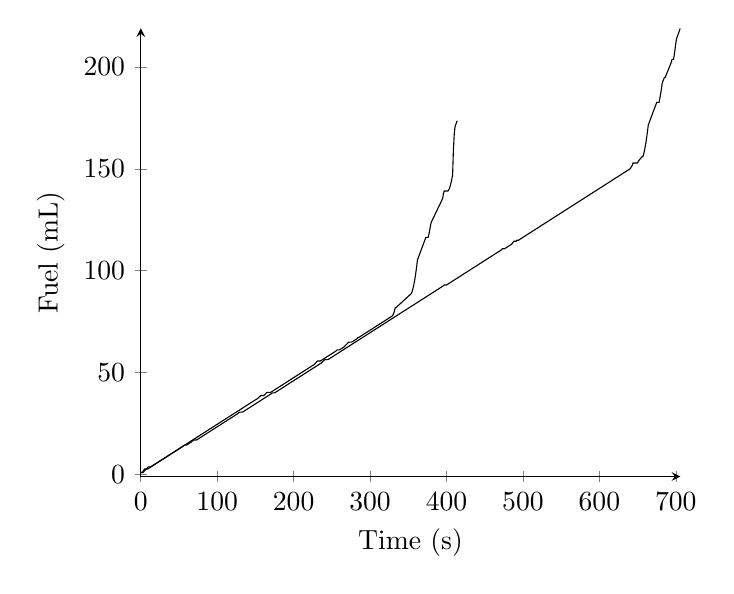
\begin{tikzpicture}
\begin{axis}[
legend style={anchor=west},
axis x line=bottom,
axis y line=left,
ymin=-1,
xlabel=Time (s),
ylabel=Fuel (mL),
]
\addplot[] coordinates {
(0, 1.00398986302)
(1, 1.00398986302)
(2, 1.00398986302)
(3, 1.00398986302)
(4, 1.39515894117)
(5, 1.78752409557)
(6, 2.18121563042)
(7, 2.57638382676)
(8, 2.97320299782)
(9, 3.37187659311)
(10, 3.77264368734)
(11, 3.77264368734)
(12, 3.77264368734)
(13, 3.77264368734)
(14, 4.0125292007)
(15, 4.25241471406)
(16, 4.49230022743)
(17, 4.73218574079)
(18, 4.97207125415)
(19, 5.21195676751)
(20, 5.45184228087)
(21, 5.69172779423)
(22, 5.93161330759)
(23, 6.17149882096)
(24, 6.41138433432)
(25, 6.65126984768)
(26, 6.89115536104)
(27, 7.1310408744)
(28, 7.37092638776)
(29, 7.61081190112)
(30, 7.85069741449)
(31, 8.09058292785)
(32, 8.33046844121)
(33, 8.57035395457)
(34, 8.81023946793)
(35, 9.05012498129)
(36, 9.29001049465)
(37, 9.52989600802)
(38, 9.76978152138)
(39, 10.0096670347)
(40, 10.2495525481)
(41, 10.4894380615)
(42, 10.7293235748)
(43, 10.9692090882)
(44, 11.2090946015)
(45, 11.4489801149)
(46, 11.6888656283)
(47, 11.9287511416)
(48, 12.168636655)
(49, 12.4085221684)
(50, 12.6484076817)
(51, 12.8882931951)
(52, 13.1281787084)
(53, 13.3680642218)
(54, 13.6079497352)
(55, 13.8478352485)
(56, 14.0877207619)
(57, 14.3276062752)
(58, 14.5674917886)
(59, 14.807377302)
(60, 15.0472628153)
(61, 15.2871483287)
(62, 15.5270338421)
(63, 15.7669193554)
(64, 16.0068048688)
(65, 16.2466903821)
(66, 16.4865758955)
(67, 16.7264614089)
(68, 16.9663469222)
(69, 17.2062324356)
(70, 17.4461179489)
(71, 17.6860034623)
(72, 17.9258889757)
(73, 18.165774489)
(74, 18.4056600024)
(75, 18.6455455158)
(76, 18.8854310291)
(77, 19.1253165425)
(78, 19.3652020558)
(79, 19.6050875692)
(80, 19.8449730826)
(81, 20.0848585959)
(82, 20.3247441093)
(83, 20.5646296226)
(84, 20.804515136)
(85, 21.0444006494)
(86, 21.2842861627)
(87, 21.5241716761)
(88, 21.7640571895)
(89, 22.0039427028)
(90, 22.2438282162)
(91, 22.4837137295)
(92, 22.7235992429)
(93, 22.9634847563)
(94, 23.2033702696)
(95, 23.443255783)
(96, 23.6831412963)
(97, 23.9230268097)
(98, 24.1629123231)
(99, 24.4027978364)
(100, 24.6426833498)
(101, 24.8825688631)
(102, 25.1224543765)
(103, 25.3623398899)
(104, 25.6022254032)
(105, 25.8421109166)
(106, 26.08199643)
(107, 26.3218819433)
(108, 26.5617674567)
(109, 26.80165297)
(110, 27.0415384834)
(111, 27.2814239968)
(112, 27.5213095101)
(113, 27.7611950235)
(114, 28.0010805368)
(115, 28.2409660502)
(116, 28.4808515636)
(117, 28.7207370769)
(118, 28.9606225903)
(119, 29.2005081037)
(120, 29.440393617)
(121, 29.6802791304)
(122, 29.9201646437)
(123, 30.1600501571)
(124, 30.3999356705)
(125, 30.6398211838)
(126, 30.8797066972)
(127, 31.1195922105)
(128, 31.3594777239)
(129, 31.5993632373)
(130, 31.8392487506)
(131, 32.079134264)
(132, 32.3190197774)
(133, 32.5589052907)
(134, 32.7987908041)
(135, 33.0386763174)
(136, 33.2785618308)
(137, 33.5184473442)
(138, 33.7583328575)
(139, 33.9982183709)
(140, 34.2381038842)
(141, 34.4779893976)
(142, 34.717874911)
(143, 34.9577604243)
(144, 35.1976459377)
(145, 35.4375314511)
(146, 35.6774169644)
(147, 35.9173024778)
(148, 36.1571879911)
(149, 36.3970735045)
(150, 36.6369590179)
(151, 36.8768445312)
(152, 37.1167300446)
(153, 37.3566155579)
(154, 37.6754102861)
(155, 38.0214797797)
(156, 38.3982514099)
(157, 38.7773300426)
(158, 38.7773300426)
(159, 38.7773300426)
(160, 38.7773300426)
(161, 38.7773300426)
(162, 39.1131872874)
(163, 39.4863461167)
(164, 39.9107983425)
(165, 40.3354002584)
(166, 40.3354002584)
(167, 40.3354002584)
(168, 40.3354002584)
(169, 40.3354002584)
(170, 40.3354002584)
(171, 40.5752857718)
(172, 40.8151712852)
(173, 41.0550567985)
(174, 41.2949423119)
(175, 41.5348278252)
(176, 41.7747133386)
(177, 42.014598852)
(178, 42.2544843653)
(179, 42.4943698787)
(180, 42.7342553921)
(181, 42.9741409054)
(182, 43.2140264188)
(183, 43.4539119321)
(184, 43.6937974455)
(185, 43.9336829589)
(186, 44.1735684722)
(187, 44.4134539856)
(188, 44.6533394989)
(189, 44.8932250123)
(190, 45.1331105257)
(191, 45.372996039)
(192, 45.6128815524)
(193, 45.8527670657)
(194, 46.0926525791)
(195, 46.3325380925)
(196, 46.5724236058)
(197, 46.8123091192)
(198, 47.0521946326)
(199, 47.2920801459)
(200, 47.5319656593)
(201, 47.7718511726)
(202, 48.011736686)
(203, 48.2516221994)
(204, 48.4915077127)
(205, 48.7313932261)
(206, 48.9712787394)
(207, 49.2111642528)
(208, 49.4510497662)
(209, 49.6909352795)
(210, 49.9308207929)
(211, 50.1707063063)
(212, 50.4105918196)
(213, 50.650477333)
(214, 50.8903628463)
(215, 51.1302483597)
(216, 51.3701338731)
(217, 51.6100193864)
(218, 51.8499048998)
(219, 52.0897904131)
(220, 52.3296759265)
(221, 52.5695614399)
(222, 52.8094469532)
(223, 53.0493324666)
(224, 53.28921798)
(225, 53.5291034933)
(226, 53.7689890067)
(227, 54.00887452)
(228, 54.3739405963)
(229, 54.7907220772)
(230, 55.2962563616)
(231, 55.7224306275)
(232, 55.7224306275)
(233, 55.7224306275)
(234, 55.7224306275)
(235, 55.7224306275)
(236, 55.9623161409)
(237, 56.2022016542)
(238, 56.4420871676)
(239, 56.681972681)
(240, 56.9218581943)
(241, 57.1617437077)
(242, 57.401629221)
(243, 57.6415147344)
(244, 57.8814002478)
(245, 58.1212857611)
(246, 58.3611712745)
(247, 58.6010567878)
(248, 58.8409423012)
(249, 59.0808278146)
(250, 59.3207133279)
(251, 59.5605988413)
(252, 59.8004843547)
(253, 60.040369868)
(254, 60.2802553814)
(255, 60.5201408947)
(256, 60.7600264081)
(257, 61.1665134408)
(258, 61.1665134408)
(259, 61.1665134408)
(260, 61.1665134408)
(261, 61.4063989542)
(262, 61.6462844675)
(263, 61.8861699809)
(264, 62.1260554942)
(265, 62.3659410076)
(266, 62.605826521)
(267, 63.0166362229)
(268, 63.4078408696)
(269, 63.7760199084)
(270, 64.1385374737)
(271, 64.6014662819)
(272, 64.993525959)
(273, 64.993525959)
(274, 64.993525959)
(275, 64.993525959)
(276, 64.993525959)
(277, 65.2334114723)
(278, 65.4732969857)
(279, 65.7131824991)
(280, 65.9530680124)
(281, 66.1929535258)
(282, 66.4328390391)
(283, 66.6727245525)
(284, 67.2382231329)
(285, 67.2382231329)
(286, 67.4781086463)
(287, 67.7179941596)
(288, 67.957879673)
(289, 68.1977651864)
(290, 68.4376506997)
(291, 68.6775362131)
(292, 68.9174217264)
(293, 69.1573072398)
(294, 69.3971927532)
(295, 69.6370782665)
(296, 69.8769637799)
(297, 70.1168492933)
(298, 70.3567348066)
(299, 70.59662032)
(300, 70.8365058333)
(301, 71.0763913467)
(302, 71.3162768601)
(303, 71.5561623734)
(304, 71.7960478868)
(305, 72.0359334001)
(306, 72.2758189135)
(307, 72.5157044269)
(308, 72.7555899402)
(309, 72.9954754536)
(310, 73.235360967)
(311, 73.4752464803)
(312, 73.7151319937)
(313, 73.955017507)
(314, 74.1949030204)
(315, 74.4347885338)
(316, 74.6746740471)
(317, 74.9145595605)
(318, 75.1544450738)
(319, 75.3943305872)
(320, 75.6342161006)
(321, 75.8741016139)
(322, 76.1139871273)
(323, 76.3538726407)
(324, 76.593758154)
(325, 76.8336436674)
(326, 77.0735291807)
(327, 77.3134146941)
(328, 77.5533002075)
(329, 77.7931857208)
(330, 78.3586843012)
(331, 79.2433215389)
(332, 80.4430316923)
(333, 81.9561576881)
(334, 81.9561576881)
(335, 82.2983700713)
(336, 82.6405956491)
(337, 82.9828364747)
(338, 83.32509505)
(339, 83.6673744553)
(340, 84.0096785264)
(341, 84.3520121024)
(342, 84.6943757251)
(343, 85.0368957377)
(344, 85.3793951584)
(345, 85.7219634925)
(346, 86.0646208839)
(347, 86.4073962379)
(348, 86.7503326381)
(349, 87.0934974511)
(350, 87.4370028071)
(351, 87.781052092)
(352, 88.1260643712)
(353, 88.4731095639)
(354, 88.8265351434)
(355, 89.79628684)
(356, 91.0804284578)
(357, 92.6779513154)
(358, 94.590255399)
(359, 96.8211493635)
(360, 99.3768505317)
(361, 102.265984895)
(362, 105.340332541)
(363, 106.344322404)
(364, 107.348312267)
(365, 108.35230213)
(366, 109.356291993)
(367, 110.360281856)
(368, 111.364271719)
(369, 112.368261582)
(370, 113.372251445)
(371, 114.376241308)
(372, 115.380231171)
(373, 116.384221035)
(374, 116.384221035)
(375, 116.384221035)
(376, 116.384221035)
(377, 117.983616297)
(378, 119.897808375)
(379, 122.130620299)
(380, 123.758840511)
(381, 124.537038064)
(382, 125.315398648)
(383, 126.093958488)
(384, 126.872764897)
(385, 127.651880729)
(386, 128.43139109)
(387, 129.21141375)
(388, 130.00345177)
(389, 130.783044079)
(390, 131.562774005)
(391, 132.342703216)
(392, 133.122933708)
(393, 133.903645094)
(394, 134.685180356)
(395, 135.46801956)
(396, 137.907749419)
(397, 139.114437489)
(398, 139.114437489)
(399, 139.114437489)
(400, 139.114437489)
(401, 139.114437489)
(402, 139.114437489)
(403, 139.679936069)
(404, 140.564573307)
(405, 141.76428346)
(406, 143.277409456)
(407, 145.104702889)
(408, 147.249324022)
(409, 159.067779967)
(410, 166.417953869)
(411, 170.270438334)
(412, 171.619915219)
(413, 172.623905082)
(414, 173.627894945)
};
\addplot[] coordinates {
(0, 1.00398986302)
(1, 1.00398986302)
(2, 1.00398986302)
(3, 1.56220432482)
(4, 2.12998612821)
(5, 2.71016271768)
(6, 2.71016271768)
(7, 2.71016271768)
(8, 2.71016271768)
(9, 2.71016271768)
(10, 2.95004823104)
(11, 3.18993374441)
(12, 3.42981925777)
(13, 3.66970477113)
(14, 3.90959028449)
(15, 4.14947579785)
(16, 4.38936131121)
(17, 4.62924682458)
(18, 4.86913233794)
(19, 5.1090178513)
(20, 5.34890336466)
(21, 5.58878887802)
(22, 5.82867439138)
(23, 6.06855990474)
(24, 6.30844541811)
(25, 6.54833093147)
(26, 6.78821644483)
(27, 7.02810195819)
(28, 7.26798747155)
(29, 7.50787298491)
(30, 7.74775849827)
(31, 7.98764401164)
(32, 8.227529525)
(33, 8.46741503836)
(34, 8.70730055172)
(35, 8.94718606508)
(36, 9.18707157844)
(37, 9.4269570918)
(38, 9.66684260517)
(39, 9.90672811853)
(40, 10.1466136319)
(41, 10.3864991453)
(42, 10.6263846586)
(43, 10.866270172)
(44, 11.1061556853)
(45, 11.3460411987)
(46, 11.5859267121)
(47, 11.8258122254)
(48, 12.0656977388)
(49, 12.3055832521)
(50, 12.5454687655)
(51, 12.7853542789)
(52, 13.0252397922)
(53, 13.2651253056)
(54, 13.5050108189)
(55, 13.8135613533)
(56, 14.1412035385)
(57, 14.4479651751)
(58, 14.4479651751)
(59, 14.4479651751)
(60, 14.4479651751)
(61, 14.6878506885)
(62, 14.9277362018)
(63, 15.1676217152)
(64, 15.4075072286)
(65, 15.6473927419)
(66, 15.8872782553)
(67, 16.2136550252)
(68, 16.5665482079)
(69, 16.938787415)
(70, 16.938787415)
(71, 16.938787415)
(72, 16.938787415)
(73, 16.938787415)
(74, 17.1786729284)
(75, 17.4185584418)
(76, 17.6584439551)
(77, 17.8983294685)
(78, 18.1382149819)
(79, 18.3781004952)
(80, 18.6179860086)
(81, 18.8578715219)
(82, 19.0977570353)
(83, 19.3376425487)
(84, 19.577528062)
(85, 19.8174135754)
(86, 20.0572990887)
(87, 20.2971846021)
(88, 20.5370701155)
(89, 20.7769556288)
(90, 21.0168411422)
(91, 21.2567266556)
(92, 21.4966121689)
(93, 21.7364976823)
(94, 21.9763831956)
(95, 22.216268709)
(96, 22.4561542224)
(97, 22.6960397357)
(98, 22.9359252491)
(99, 23.1758107624)
(100, 23.4156962758)
(101, 23.6555817892)
(102, 23.8954673025)
(103, 24.1353528159)
(104, 24.3752383293)
(105, 24.6151238426)
(106, 24.855009356)
(107, 25.0948948693)
(108, 25.3347803827)
(109, 25.5746658961)
(110, 25.8145514094)
(111, 26.0544369228)
(112, 26.2943224361)
(113, 26.5342079495)
(114, 26.7740934629)
(115, 27.0139789762)
(116, 27.2538644896)
(117, 27.493750003)
(118, 27.7336355163)
(119, 27.9735210297)
(120, 28.213406543)
(121, 28.4532920564)
(122, 28.6931775698)
(123, 28.9330630831)
(124, 29.1729485965)
(125, 29.4128341098)
(126, 29.6527196232)
(127, 29.8926051366)
(128, 30.2295784714)
(129, 30.5816510348)
(130, 30.5816510348)
(131, 30.5816510348)
(132, 30.5816510348)
(133, 30.5816510348)
(134, 30.8215365482)
(135, 31.0614220615)
(136, 31.3013075749)
(137, 31.5411930882)
(138, 31.7810786016)
(139, 32.020964115)
(140, 32.2608496283)
(141, 32.5007351417)
(142, 32.740620655)
(143, 32.9805061684)
(144, 33.2203916818)
(145, 33.4602771951)
(146, 33.7001627085)
(147, 33.9400482219)
(148, 34.1799337352)
(149, 34.4198192486)
(150, 34.6597047619)
(151, 34.8995902753)
(152, 35.1394757887)
(153, 35.379361302)
(154, 35.6192468154)
(155, 35.8591323287)
(156, 36.0990178421)
(157, 36.3389033555)
(158, 36.5787888688)
(159, 36.8186743822)
(160, 37.0585598956)
(161, 37.2984454089)
(162, 37.5383309223)
(163, 37.7782164356)
(164, 38.018101949)
(165, 38.2579874624)
(166, 38.4978729757)
(167, 38.7377584891)
(168, 38.9776440024)
(169, 39.2175295158)
(170, 39.4574150292)
(171, 39.6973005425)
(172, 40.0462181687)
(173, 40.0462181687)
(174, 40.0462181687)
(175, 40.0462181687)
(176, 40.286103682)
(177, 40.5259891954)
(178, 40.7658747088)
(179, 41.0057602221)
(180, 41.2456457355)
(181, 41.4855312488)
(182, 41.7254167622)
(183, 41.9653022756)
(184, 42.2051877889)
(185, 42.4450733023)
(186, 42.6849588156)
(187, 42.924844329)
(188, 43.1647298424)
(189, 43.4046153557)
(190, 43.6445008691)
(191, 43.8843863825)
(192, 44.1242718958)
(193, 44.3641574092)
(194, 44.6040429225)
(195, 44.8439284359)
(196, 45.0838139493)
(197, 45.3236994626)
(198, 45.563584976)
(199, 45.8034704893)
(200, 46.0433560027)
(201, 46.2832415161)
(202, 46.5231270294)
(203, 46.7630125428)
(204, 47.0028980562)
(205, 47.2427835695)
(206, 47.4826690829)
(207, 47.7225545962)
(208, 47.9624401096)
(209, 48.202325623)
(210, 48.4422111363)
(211, 48.6820966497)
(212, 48.921982163)
(213, 49.1618676764)
(214, 49.4017531898)
(215, 49.6416387031)
(216, 49.8815242165)
(217, 50.1214097299)
(218, 50.3612952432)
(219, 50.6011807566)
(220, 50.8410662699)
(221, 51.0809517833)
(222, 51.3208372967)
(223, 51.56072281)
(224, 51.8006083234)
(225, 52.0404938367)
(226, 52.2803793501)
(227, 52.5202648635)
(228, 52.7601503768)
(229, 53.0000358902)
(230, 53.2399214036)
(231, 53.4798069169)
(232, 53.7196924303)
(233, 53.9595779436)
(234, 54.199463457)
(235, 54.4393489704)
(236, 54.6792344837)
(237, 55.0280182903)
(238, 55.420201219)
(239, 55.7482252469)
(240, 56.0761294264)
(241, 56.4051411833)
(242, 56.4051411833)
(243, 56.4051411833)
(244, 56.4051411833)
(245, 56.4051411833)
(246, 56.6450266966)
(247, 56.88491221)
(248, 57.1247977234)
(249, 57.3646832367)
(250, 57.6045687501)
(251, 57.8444542634)
(252, 58.0843397768)
(253, 58.3242252902)
(254, 58.5641108035)
(255, 58.8039963169)
(256, 59.0438818302)
(257, 59.2837673436)
(258, 59.523652857)
(259, 59.7635383703)
(260, 60.0034238837)
(261, 60.243309397)
(262, 60.4831949104)
(263, 60.7230804238)
(264, 60.9629659371)
(265, 61.2028514505)
(266, 61.4427369639)
(267, 61.6826224772)
(268, 61.9225079906)
(269, 62.1623935039)
(270, 62.4022790173)
(271, 62.6421645307)
(272, 62.882050044)
(273, 63.1219355574)
(274, 63.3618210707)
(275, 63.6017065841)
(276, 63.8415920975)
(277, 64.0814776108)
(278, 64.3213631242)
(279, 64.5612486376)
(280, 64.8011341509)
(281, 65.0410196643)
(282, 65.2809051776)
(283, 65.520790691)
(284, 65.7606762044)
(285, 66.0005617177)
(286, 66.2404472311)
(287, 66.4803327444)
(288, 66.7202182578)
(289, 66.9601037712)
(290, 67.1999892845)
(291, 67.4398747979)
(292, 67.6797603113)
(293, 67.9196458246)
(294, 68.159531338)
(295, 68.3994168513)
(296, 68.6393023647)
(297, 68.8791878781)
(298, 69.1190733914)
(299, 69.3589589048)
(300, 69.5988444181)
(301, 69.8387299315)
(302, 70.0786154449)
(303, 70.3185009582)
(304, 70.5583864716)
(305, 70.798271985)
(306, 71.0381574983)
(307, 71.2780430117)
(308, 71.517928525)
(309, 71.7578140384)
(310, 71.9976995518)
(311, 72.2375850651)
(312, 72.4774705785)
(313, 72.7173560918)
(314, 72.9572416052)
(315, 73.1971271186)
(316, 73.4370126319)
(317, 73.6768981453)
(318, 73.9167836587)
(319, 74.156669172)
(320, 74.3965546854)
(321, 74.6364401987)
(322, 74.8763257121)
(323, 75.1162112255)
(324, 75.3560967388)
(325, 75.5959822522)
(326, 75.8358677655)
(327, 76.0757532789)
(328, 76.3156387923)
(329, 76.5555243056)
(330, 76.795409819)
(331, 77.0352953324)
(332, 77.2751808457)
(333, 77.5150663591)
(334, 77.7549518724)
(335, 77.9948373858)
(336, 78.2347228992)
(337, 78.4746084125)
(338, 78.7144939259)
(339, 78.9543794392)
(340, 79.1942649526)
(341, 79.434150466)
(342, 79.6740359793)
(343, 79.9139214927)
(344, 80.1538070061)
(345, 80.3936925194)
(346, 80.6335780328)
(347, 80.8734635461)
(348, 81.1133490595)
(349, 81.3532345729)
(350, 81.5931200862)
(351, 81.8330055996)
(352, 82.0728911129)
(353, 82.3127766263)
(354, 82.5526621397)
(355, 82.792547653)
(356, 83.0324331664)
(357, 83.2723186798)
(358, 83.5122041931)
(359, 83.7520897065)
(360, 83.9919752198)
(361, 84.2318607332)
(362, 84.4717462466)
(363, 84.7116317599)
(364, 84.9515172733)
(365, 85.1914027866)
(366, 85.4312883)
(367, 85.6711738134)
(368, 85.9110593267)
(369, 86.1509448401)
(370, 86.3908303534)
(371, 86.6307158668)
(372, 86.8706013802)
(373, 87.1104868935)
(374, 87.3503724069)
(375, 87.5902579203)
(376, 87.8301434336)
(377, 88.070028947)
(378, 88.3099144603)
(379, 88.5497999737)
(380, 88.7896854871)
(381, 89.0295710004)
(382, 89.2694565138)
(383, 89.5093420271)
(384, 89.7492275405)
(385, 89.9891130539)
(386, 90.2289985672)
(387, 90.4688840806)
(388, 90.708769594)
(389, 90.9486551073)
(390, 91.1885406207)
(391, 91.428426134)
(392, 91.6683116474)
(393, 91.9081971608)
(394, 92.1480826741)
(395, 92.3879681875)
(396, 92.6278537008)
(397, 93.0127159839)
(398, 93.0127159839)
(399, 93.0127159839)
(400, 93.0127159839)
(401, 93.2526014972)
(402, 93.4924870106)
(403, 93.732372524)
(404, 93.9722580373)
(405, 94.2121435507)
(406, 94.452029064)
(407, 94.6919145774)
(408, 94.9318000908)
(409, 95.1716856041)
(410, 95.4115711175)
(411, 95.6514566308)
(412, 95.8913421442)
(413, 96.1312276576)
(414, 96.3711131709)
(415, 96.6109986843)
(416, 96.8508841977)
(417, 97.090769711)
(418, 97.3306552244)
(419, 97.5705407377)
(420, 97.8104262511)
(421, 98.0503117645)
(422, 98.2901972778)
(423, 98.5300827912)
(424, 98.7699683045)
(425, 99.0098538179)
(426, 99.2497393313)
(427, 99.4896248446)
(428, 99.729510358)
(429, 99.9693958714)
(430, 100.209281385)
(431, 100.449166898)
(432, 100.689052411)
(433, 100.928937925)
(434, 101.168823438)
(435, 101.408708952)
(436, 101.648594465)
(437, 101.888479978)
(438, 102.128365492)
(439, 102.368251005)
(440, 102.608136518)
(441, 102.848022032)
(442, 103.087907545)
(443, 103.327793058)
(444, 103.567678572)
(445, 103.807564085)
(446, 104.047449598)
(447, 104.287335112)
(448, 104.527220625)
(449, 104.767106139)
(450, 105.006991652)
(451, 105.246877165)
(452, 105.486762679)
(453, 105.726648192)
(454, 105.966533705)
(455, 106.206419219)
(456, 106.446304732)
(457, 106.686190245)
(458, 106.926075759)
(459, 107.165961272)
(460, 107.405846786)
(461, 107.645732299)
(462, 107.885617812)
(463, 108.125503326)
(464, 108.365388839)
(465, 108.605274352)
(466, 108.845159866)
(467, 109.085045379)
(468, 109.324930892)
(469, 109.564816406)
(470, 109.804701919)
(471, 110.044587433)
(472, 110.428992117)
(473, 110.805973467)
(474, 110.805973467)
(475, 110.805973467)
(476, 110.805973467)
(477, 111.04585898)
(478, 111.285744493)
(479, 111.525630007)
(480, 111.76551552)
(481, 112.005401033)
(482, 112.245286547)
(483, 112.48517206)
(484, 112.725057574)
(485, 112.964943087)
(486, 113.376162188)
(487, 113.873501298)
(488, 114.481196488)
(489, 114.481196488)
(490, 114.481196488)
(491, 114.481196488)
(492, 114.95345684)
(493, 114.95345684)
(494, 114.95345684)
(495, 115.193342353)
(496, 115.433227866)
(497, 115.67311338)
(498, 115.912998893)
(499, 116.152884406)
(500, 116.39276992)
(501, 116.632655433)
(502, 116.872540946)
(503, 117.11242646)
(504, 117.352311973)
(505, 117.592197487)
(506, 117.832083)
(507, 118.071968513)
(508, 118.311854027)
(509, 118.55173954)
(510, 118.791625053)
(511, 119.031510567)
(512, 119.27139608)
(513, 119.511281593)
(514, 119.751167107)
(515, 119.99105262)
(516, 120.230938134)
(517, 120.470823647)
(518, 120.71070916)
(519, 120.950594674)
(520, 121.190480187)
(521, 121.4303657)
(522, 121.670251214)
(523, 121.910136727)
(524, 122.15002224)
(525, 122.389907754)
(526, 122.629793267)
(527, 122.869678781)
(528, 123.109564294)
(529, 123.349449807)
(530, 123.589335321)
(531, 123.829220834)
(532, 124.069106347)
(533, 124.308991861)
(534, 124.548877374)
(535, 124.788762887)
(536, 125.028648401)
(537, 125.268533914)
(538, 125.508419427)
(539, 125.748304941)
(540, 125.988190454)
(541, 126.228075968)
(542, 126.467961481)
(543, 126.707846994)
(544, 126.947732508)
(545, 127.187618021)
(546, 127.427503534)
(547, 127.667389048)
(548, 127.907274561)
(549, 128.147160074)
(550, 128.387045588)
(551, 128.626931101)
(552, 128.866816615)
(553, 129.106702128)
(554, 129.346587641)
(555, 129.586473155)
(556, 129.826358668)
(557, 130.066244181)
(558, 130.306129695)
(559, 130.546015208)
(560, 130.785900721)
(561, 131.025786235)
(562, 131.265671748)
(563, 131.505557262)
(564, 131.745442775)
(565, 131.985328288)
(566, 132.225213802)
(567, 132.465099315)
(568, 132.704984828)
(569, 132.944870342)
(570, 133.184755855)
(571, 133.424641368)
(572, 133.664526882)
(573, 133.904412395)
(574, 134.144297908)
(575, 134.384183422)
(576, 134.624068935)
(577, 134.863954449)
(578, 135.103839962)
(579, 135.343725475)
(580, 135.583610989)
(581, 135.823496502)
(582, 136.063382015)
(583, 136.303267529)
(584, 136.543153042)
(585, 136.783038555)
(586, 137.022924069)
(587, 137.262809582)
(588, 137.502695096)
(589, 137.742580609)
(590, 137.982466122)
(591, 138.222351636)
(592, 138.462237149)
(593, 138.702122662)
(594, 138.942008176)
(595, 139.181893689)
(596, 139.421779202)
(597, 139.661664716)
(598, 139.901550229)
(599, 140.141435743)
(600, 140.381321256)
(601, 140.621206769)
(602, 140.861092283)
(603, 141.100977796)
(604, 141.340863309)
(605, 141.580748823)
(606, 141.820634336)
(607, 142.060519849)
(608, 142.300405363)
(609, 142.540290876)
(610, 142.78017639)
(611, 143.020061903)
(612, 143.259947416)
(613, 143.49983293)
(614, 143.739718443)
(615, 143.979603956)
(616, 144.21948947)
(617, 144.459374983)
(618, 144.699260496)
(619, 144.93914601)
(620, 145.179031523)
(621, 145.418917036)
(622, 145.65880255)
(623, 145.898688063)
(624, 146.138573577)
(625, 146.37845909)
(626, 146.618344603)
(627, 146.858230117)
(628, 147.09811563)
(629, 147.338001143)
(630, 147.577886657)
(631, 147.81777217)
(632, 148.057657683)
(633, 148.297543197)
(634, 148.53742871)
(635, 148.777314224)
(636, 149.017199737)
(637, 149.25708525)
(638, 149.496970764)
(639, 149.736856277)
(640, 149.97674179)
(641, 150.472180293)
(642, 151.154140033)
(643, 151.685004764)
(644, 152.894087411)
(645, 152.894087411)
(646, 152.894087411)
(647, 152.894087411)
(648, 152.894087411)
(649, 152.894087411)
(650, 152.894087411)
(651, 153.798361732)
(652, 154.249845037)
(653, 154.702265904)
(654, 155.155101242)
(655, 155.609558032)
(656, 156.068036742)
(657, 156.068036742)
(658, 157.370761926)
(659, 158.986884183)
(660, 160.917946299)
(661, 163.16789973)
(662, 165.743104598)
(663, 168.652329696)
(664, 171.552107284)
(665, 172.556097147)
(666, 173.56008701)
(667, 174.564076873)
(668, 175.568066736)
(669, 176.572056599)
(670, 177.576046462)
(671, 178.580036325)
(672, 179.584026188)
(673, 180.588016051)
(674, 181.592005914)
(675, 182.595995777)
(676, 182.595995777)
(677, 182.595995777)
(678, 182.595995777)
(679, 184.358877575)
(680, 186.438245051)
(681, 188.83917467)
(682, 191.569151567)
(683, 192.949218616)
(684, 193.841802856)
(685, 194.847525197)
(686, 194.847525197)
(687, 195.765539893)
(688, 196.685040856)
(689, 197.605908091)
(690, 198.523001034)
(691, 199.441058808)
(692, 200.360673408)
(693, 201.282992658)
(694, 202.210512329)
(695, 203.757183275)
(696, 203.757183275)
(697, 203.757183275)
(698, 206.082005509)
(699, 208.733900597)
(700, 211.722196625)
(701, 213.998175848)
(702, 215.002165711)
(703, 216.006155574)
(704, 217.010145437)
(705, 218.0141353)
(706, 219.018125163)
};

\end{axis}
\end{tikzpicture}
\label{tik:fuel:100:51}
\caption{100 percent diving with GSC on route $51$}
\end{figure}

%
\begin{figure}
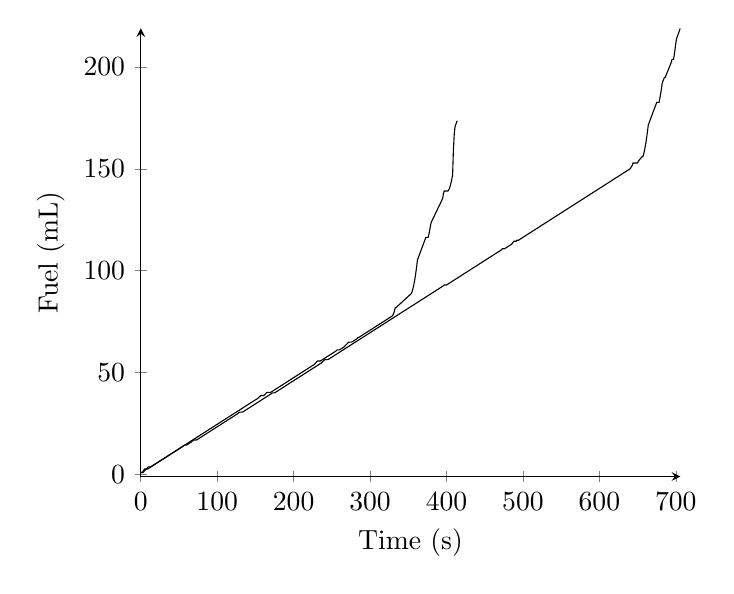
\begin{tikzpicture}
\begin{axis}[
legend style={anchor=west},
axis x line=bottom,
axis y line=left,
ymin=-1,
xlabel=Time (s),
ylabel=Fuel (mL),
]
\addplot[] coordinates {
(0, 1.00398986302)
(1, 1.00398986302)
(2, 1.00398986302)
(3, 1.00398986302)
(4, 1.39515894117)
(5, 1.78752409557)
(6, 2.18121563042)
(7, 2.57638382676)
(8, 2.97320299782)
(9, 3.37187659311)
(10, 3.77264368734)
(11, 3.77264368734)
(12, 3.77264368734)
(13, 3.77264368734)
(14, 4.0125292007)
(15, 4.25241471406)
(16, 4.49230022743)
(17, 4.73218574079)
(18, 4.97207125415)
(19, 5.21195676751)
(20, 5.45184228087)
(21, 5.69172779423)
(22, 5.93161330759)
(23, 6.17149882096)
(24, 6.41138433432)
(25, 6.65126984768)
(26, 6.89115536104)
(27, 7.1310408744)
(28, 7.37092638776)
(29, 7.61081190112)
(30, 7.85069741449)
(31, 8.09058292785)
(32, 8.33046844121)
(33, 8.57035395457)
(34, 8.81023946793)
(35, 9.05012498129)
(36, 9.29001049465)
(37, 9.52989600802)
(38, 9.76978152138)
(39, 10.0096670347)
(40, 10.2495525481)
(41, 10.4894380615)
(42, 10.7293235748)
(43, 10.9692090882)
(44, 11.2090946015)
(45, 11.4489801149)
(46, 11.6888656283)
(47, 11.9287511416)
(48, 12.168636655)
(49, 12.4085221684)
(50, 12.6484076817)
(51, 12.8882931951)
(52, 13.1281787084)
(53, 13.3680642218)
(54, 13.6079497352)
(55, 13.8478352485)
(56, 14.0877207619)
(57, 14.3276062752)
(58, 14.5674917886)
(59, 14.807377302)
(60, 15.0472628153)
(61, 15.2871483287)
(62, 15.5270338421)
(63, 15.7669193554)
(64, 16.0068048688)
(65, 16.2466903821)
(66, 16.4865758955)
(67, 16.7264614089)
(68, 16.9663469222)
(69, 17.2062324356)
(70, 17.4461179489)
(71, 17.6860034623)
(72, 17.9258889757)
(73, 18.165774489)
(74, 18.4056600024)
(75, 18.6455455158)
(76, 18.8854310291)
(77, 19.1253165425)
(78, 19.3652020558)
(79, 19.6050875692)
(80, 19.8449730826)
(81, 20.0848585959)
(82, 20.3247441093)
(83, 20.5646296226)
(84, 20.804515136)
(85, 21.0444006494)
(86, 21.2842861627)
(87, 21.5241716761)
(88, 21.7640571895)
(89, 22.0039427028)
(90, 22.2438282162)
(91, 22.4837137295)
(92, 22.7235992429)
(93, 22.9634847563)
(94, 23.2033702696)
(95, 23.443255783)
(96, 23.6831412963)
(97, 23.9230268097)
(98, 24.1629123231)
(99, 24.4027978364)
(100, 24.6426833498)
(101, 24.8825688631)
(102, 25.1224543765)
(103, 25.3623398899)
(104, 25.6022254032)
(105, 25.8421109166)
(106, 26.08199643)
(107, 26.3218819433)
(108, 26.5617674567)
(109, 26.80165297)
(110, 27.0415384834)
(111, 27.2814239968)
(112, 27.5213095101)
(113, 27.7611950235)
(114, 28.0010805368)
(115, 28.2409660502)
(116, 28.4808515636)
(117, 28.7207370769)
(118, 28.9606225903)
(119, 29.2005081037)
(120, 29.440393617)
(121, 29.6802791304)
(122, 29.9201646437)
(123, 30.1600501571)
(124, 30.3999356705)
(125, 30.6398211838)
(126, 30.8797066972)
(127, 31.1195922105)
(128, 31.3594777239)
(129, 31.5993632373)
(130, 31.8392487506)
(131, 32.079134264)
(132, 32.3190197774)
(133, 32.5589052907)
(134, 32.7987908041)
(135, 33.0386763174)
(136, 33.2785618308)
(137, 33.5184473442)
(138, 33.7583328575)
(139, 33.9982183709)
(140, 34.2381038842)
(141, 34.4779893976)
(142, 34.717874911)
(143, 34.9577604243)
(144, 35.1976459377)
(145, 35.4375314511)
(146, 35.6774169644)
(147, 35.9173024778)
(148, 36.1571879911)
(149, 36.3970735045)
(150, 36.6369590179)
(151, 36.8768445312)
(152, 37.1167300446)
(153, 37.3566155579)
(154, 37.6754102861)
(155, 38.0214797797)
(156, 38.3982514099)
(157, 38.7773300426)
(158, 38.7773300426)
(159, 38.7773300426)
(160, 38.7773300426)
(161, 38.7773300426)
(162, 39.1131872874)
(163, 39.4863461167)
(164, 39.9107983425)
(165, 40.3354002584)
(166, 40.3354002584)
(167, 40.3354002584)
(168, 40.3354002584)
(169, 40.3354002584)
(170, 40.3354002584)
(171, 40.5752857718)
(172, 40.8151712852)
(173, 41.0550567985)
(174, 41.2949423119)
(175, 41.5348278252)
(176, 41.7747133386)
(177, 42.014598852)
(178, 42.2544843653)
(179, 42.4943698787)
(180, 42.7342553921)
(181, 42.9741409054)
(182, 43.2140264188)
(183, 43.4539119321)
(184, 43.6937974455)
(185, 43.9336829589)
(186, 44.1735684722)
(187, 44.4134539856)
(188, 44.6533394989)
(189, 44.8932250123)
(190, 45.1331105257)
(191, 45.372996039)
(192, 45.6128815524)
(193, 45.8527670657)
(194, 46.0926525791)
(195, 46.3325380925)
(196, 46.5724236058)
(197, 46.8123091192)
(198, 47.0521946326)
(199, 47.2920801459)
(200, 47.5319656593)
(201, 47.7718511726)
(202, 48.011736686)
(203, 48.2516221994)
(204, 48.4915077127)
(205, 48.7313932261)
(206, 48.9712787394)
(207, 49.2111642528)
(208, 49.4510497662)
(209, 49.6909352795)
(210, 49.9308207929)
(211, 50.1707063063)
(212, 50.4105918196)
(213, 50.650477333)
(214, 50.8903628463)
(215, 51.1302483597)
(216, 51.3701338731)
(217, 51.6100193864)
(218, 51.8499048998)
(219, 52.0897904131)
(220, 52.3296759265)
(221, 52.5695614399)
(222, 52.8094469532)
(223, 53.0493324666)
(224, 53.28921798)
(225, 53.5291034933)
(226, 53.7689890067)
(227, 54.00887452)
(228, 54.3739405963)
(229, 54.7907220772)
(230, 55.2962563616)
(231, 55.7224306275)
(232, 55.7224306275)
(233, 55.7224306275)
(234, 55.7224306275)
(235, 55.7224306275)
(236, 55.9623161409)
(237, 56.2022016542)
(238, 56.4420871676)
(239, 56.681972681)
(240, 56.9218581943)
(241, 57.1617437077)
(242, 57.401629221)
(243, 57.6415147344)
(244, 57.8814002478)
(245, 58.1212857611)
(246, 58.3611712745)
(247, 58.6010567878)
(248, 58.8409423012)
(249, 59.0808278146)
(250, 59.3207133279)
(251, 59.5605988413)
(252, 59.8004843547)
(253, 60.040369868)
(254, 60.2802553814)
(255, 60.5201408947)
(256, 60.7600264081)
(257, 61.1665134408)
(258, 61.1665134408)
(259, 61.1665134408)
(260, 61.1665134408)
(261, 61.4063989542)
(262, 61.6462844675)
(263, 61.8861699809)
(264, 62.1260554942)
(265, 62.3659410076)
(266, 62.605826521)
(267, 63.0166362229)
(268, 63.4078408696)
(269, 63.7760199084)
(270, 64.1385374737)
(271, 64.6014662819)
(272, 64.993525959)
(273, 64.993525959)
(274, 64.993525959)
(275, 64.993525959)
(276, 64.993525959)
(277, 65.2334114723)
(278, 65.4732969857)
(279, 65.7131824991)
(280, 65.9530680124)
(281, 66.1929535258)
(282, 66.4328390391)
(283, 66.6727245525)
(284, 67.2382231329)
(285, 67.2382231329)
(286, 67.4781086463)
(287, 67.7179941596)
(288, 67.957879673)
(289, 68.1977651864)
(290, 68.4376506997)
(291, 68.6775362131)
(292, 68.9174217264)
(293, 69.1573072398)
(294, 69.3971927532)
(295, 69.6370782665)
(296, 69.8769637799)
(297, 70.1168492933)
(298, 70.3567348066)
(299, 70.59662032)
(300, 70.8365058333)
(301, 71.0763913467)
(302, 71.3162768601)
(303, 71.5561623734)
(304, 71.7960478868)
(305, 72.0359334001)
(306, 72.2758189135)
(307, 72.5157044269)
(308, 72.7555899402)
(309, 72.9954754536)
(310, 73.235360967)
(311, 73.4752464803)
(312, 73.7151319937)
(313, 73.955017507)
(314, 74.1949030204)
(315, 74.4347885338)
(316, 74.6746740471)
(317, 74.9145595605)
(318, 75.1544450738)
(319, 75.3943305872)
(320, 75.6342161006)
(321, 75.8741016139)
(322, 76.1139871273)
(323, 76.3538726407)
(324, 76.593758154)
(325, 76.8336436674)
(326, 77.0735291807)
(327, 77.3134146941)
(328, 77.5533002075)
(329, 77.7931857208)
(330, 78.3586843012)
(331, 79.2433215389)
(332, 80.4430316923)
(333, 81.9561576881)
(334, 81.9561576881)
(335, 82.2983700713)
(336, 82.6405956491)
(337, 82.9828364747)
(338, 83.32509505)
(339, 83.6673744553)
(340, 84.0096785264)
(341, 84.3520121024)
(342, 84.6943757251)
(343, 85.0368957377)
(344, 85.3793951584)
(345, 85.7219634925)
(346, 86.0646208839)
(347, 86.4073962379)
(348, 86.7503326381)
(349, 87.0934974511)
(350, 87.4370028071)
(351, 87.781052092)
(352, 88.1260643712)
(353, 88.4731095639)
(354, 88.8265351434)
(355, 89.79628684)
(356, 91.0804284578)
(357, 92.6779513154)
(358, 94.590255399)
(359, 96.8211493635)
(360, 99.3768505317)
(361, 102.265984895)
(362, 105.340332541)
(363, 106.344322404)
(364, 107.348312267)
(365, 108.35230213)
(366, 109.356291993)
(367, 110.360281856)
(368, 111.364271719)
(369, 112.368261582)
(370, 113.372251445)
(371, 114.376241308)
(372, 115.380231171)
(373, 116.384221035)
(374, 116.384221035)
(375, 116.384221035)
(376, 116.384221035)
(377, 117.983616297)
(378, 119.897808375)
(379, 122.130620299)
(380, 123.758840511)
(381, 124.537038064)
(382, 125.315398648)
(383, 126.093958488)
(384, 126.872764897)
(385, 127.651880729)
(386, 128.43139109)
(387, 129.21141375)
(388, 130.00345177)
(389, 130.783044079)
(390, 131.562774005)
(391, 132.342703216)
(392, 133.122933708)
(393, 133.903645094)
(394, 134.685180356)
(395, 135.46801956)
(396, 137.907749419)
(397, 139.114437489)
(398, 139.114437489)
(399, 139.114437489)
(400, 139.114437489)
(401, 139.114437489)
(402, 139.114437489)
(403, 139.679936069)
(404, 140.564573307)
(405, 141.76428346)
(406, 143.277409456)
(407, 145.104702889)
(408, 147.249324022)
(409, 159.067779967)
(410, 166.417953869)
(411, 170.270438334)
(412, 171.619915219)
(413, 172.623905082)
(414, 173.627894945)
};
\addplot[] coordinates {
(0, 1.00398986302)
(1, 1.00398986302)
(2, 1.00398986302)
(3, 1.56220432482)
(4, 2.12998612821)
(5, 2.71016271768)
(6, 2.71016271768)
(7, 2.71016271768)
(8, 2.71016271768)
(9, 2.71016271768)
(10, 2.95004823104)
(11, 3.18993374441)
(12, 3.42981925777)
(13, 3.66970477113)
(14, 3.90959028449)
(15, 4.14947579785)
(16, 4.38936131121)
(17, 4.62924682458)
(18, 4.86913233794)
(19, 5.1090178513)
(20, 5.34890336466)
(21, 5.58878887802)
(22, 5.82867439138)
(23, 6.06855990474)
(24, 6.30844541811)
(25, 6.54833093147)
(26, 6.78821644483)
(27, 7.02810195819)
(28, 7.26798747155)
(29, 7.50787298491)
(30, 7.74775849827)
(31, 7.98764401164)
(32, 8.227529525)
(33, 8.46741503836)
(34, 8.70730055172)
(35, 8.94718606508)
(36, 9.18707157844)
(37, 9.4269570918)
(38, 9.66684260517)
(39, 9.90672811853)
(40, 10.1466136319)
(41, 10.3864991453)
(42, 10.6263846586)
(43, 10.866270172)
(44, 11.1061556853)
(45, 11.3460411987)
(46, 11.5859267121)
(47, 11.8258122254)
(48, 12.0656977388)
(49, 12.3055832521)
(50, 12.5454687655)
(51, 12.7853542789)
(52, 13.0252397922)
(53, 13.2651253056)
(54, 13.5050108189)
(55, 13.8135613533)
(56, 14.1412035385)
(57, 14.4479651751)
(58, 14.4479651751)
(59, 14.4479651751)
(60, 14.4479651751)
(61, 14.6878506885)
(62, 14.9277362018)
(63, 15.1676217152)
(64, 15.4075072286)
(65, 15.6473927419)
(66, 15.8872782553)
(67, 16.2136550252)
(68, 16.5665482079)
(69, 16.938787415)
(70, 16.938787415)
(71, 16.938787415)
(72, 16.938787415)
(73, 16.938787415)
(74, 17.1786729284)
(75, 17.4185584418)
(76, 17.6584439551)
(77, 17.8983294685)
(78, 18.1382149819)
(79, 18.3781004952)
(80, 18.6179860086)
(81, 18.8578715219)
(82, 19.0977570353)
(83, 19.3376425487)
(84, 19.577528062)
(85, 19.8174135754)
(86, 20.0572990887)
(87, 20.2971846021)
(88, 20.5370701155)
(89, 20.7769556288)
(90, 21.0168411422)
(91, 21.2567266556)
(92, 21.4966121689)
(93, 21.7364976823)
(94, 21.9763831956)
(95, 22.216268709)
(96, 22.4561542224)
(97, 22.6960397357)
(98, 22.9359252491)
(99, 23.1758107624)
(100, 23.4156962758)
(101, 23.6555817892)
(102, 23.8954673025)
(103, 24.1353528159)
(104, 24.3752383293)
(105, 24.6151238426)
(106, 24.855009356)
(107, 25.0948948693)
(108, 25.3347803827)
(109, 25.5746658961)
(110, 25.8145514094)
(111, 26.0544369228)
(112, 26.2943224361)
(113, 26.5342079495)
(114, 26.7740934629)
(115, 27.0139789762)
(116, 27.2538644896)
(117, 27.493750003)
(118, 27.7336355163)
(119, 27.9735210297)
(120, 28.213406543)
(121, 28.4532920564)
(122, 28.6931775698)
(123, 28.9330630831)
(124, 29.1729485965)
(125, 29.4128341098)
(126, 29.6527196232)
(127, 29.8926051366)
(128, 30.2295784714)
(129, 30.5816510348)
(130, 30.5816510348)
(131, 30.5816510348)
(132, 30.5816510348)
(133, 30.5816510348)
(134, 30.8215365482)
(135, 31.0614220615)
(136, 31.3013075749)
(137, 31.5411930882)
(138, 31.7810786016)
(139, 32.020964115)
(140, 32.2608496283)
(141, 32.5007351417)
(142, 32.740620655)
(143, 32.9805061684)
(144, 33.2203916818)
(145, 33.4602771951)
(146, 33.7001627085)
(147, 33.9400482219)
(148, 34.1799337352)
(149, 34.4198192486)
(150, 34.6597047619)
(151, 34.8995902753)
(152, 35.1394757887)
(153, 35.379361302)
(154, 35.6192468154)
(155, 35.8591323287)
(156, 36.0990178421)
(157, 36.3389033555)
(158, 36.5787888688)
(159, 36.8186743822)
(160, 37.0585598956)
(161, 37.2984454089)
(162, 37.5383309223)
(163, 37.7782164356)
(164, 38.018101949)
(165, 38.2579874624)
(166, 38.4978729757)
(167, 38.7377584891)
(168, 38.9776440024)
(169, 39.2175295158)
(170, 39.4574150292)
(171, 39.6973005425)
(172, 40.0462181687)
(173, 40.0462181687)
(174, 40.0462181687)
(175, 40.0462181687)
(176, 40.286103682)
(177, 40.5259891954)
(178, 40.7658747088)
(179, 41.0057602221)
(180, 41.2456457355)
(181, 41.4855312488)
(182, 41.7254167622)
(183, 41.9653022756)
(184, 42.2051877889)
(185, 42.4450733023)
(186, 42.6849588156)
(187, 42.924844329)
(188, 43.1647298424)
(189, 43.4046153557)
(190, 43.6445008691)
(191, 43.8843863825)
(192, 44.1242718958)
(193, 44.3641574092)
(194, 44.6040429225)
(195, 44.8439284359)
(196, 45.0838139493)
(197, 45.3236994626)
(198, 45.563584976)
(199, 45.8034704893)
(200, 46.0433560027)
(201, 46.2832415161)
(202, 46.5231270294)
(203, 46.7630125428)
(204, 47.0028980562)
(205, 47.2427835695)
(206, 47.4826690829)
(207, 47.7225545962)
(208, 47.9624401096)
(209, 48.202325623)
(210, 48.4422111363)
(211, 48.6820966497)
(212, 48.921982163)
(213, 49.1618676764)
(214, 49.4017531898)
(215, 49.6416387031)
(216, 49.8815242165)
(217, 50.1214097299)
(218, 50.3612952432)
(219, 50.6011807566)
(220, 50.8410662699)
(221, 51.0809517833)
(222, 51.3208372967)
(223, 51.56072281)
(224, 51.8006083234)
(225, 52.0404938367)
(226, 52.2803793501)
(227, 52.5202648635)
(228, 52.7601503768)
(229, 53.0000358902)
(230, 53.2399214036)
(231, 53.4798069169)
(232, 53.7196924303)
(233, 53.9595779436)
(234, 54.199463457)
(235, 54.4393489704)
(236, 54.6792344837)
(237, 55.0280182903)
(238, 55.420201219)
(239, 55.7482252469)
(240, 56.0761294264)
(241, 56.4051411833)
(242, 56.4051411833)
(243, 56.4051411833)
(244, 56.4051411833)
(245, 56.4051411833)
(246, 56.6450266966)
(247, 56.88491221)
(248, 57.1247977234)
(249, 57.3646832367)
(250, 57.6045687501)
(251, 57.8444542634)
(252, 58.0843397768)
(253, 58.3242252902)
(254, 58.5641108035)
(255, 58.8039963169)
(256, 59.0438818302)
(257, 59.2837673436)
(258, 59.523652857)
(259, 59.7635383703)
(260, 60.0034238837)
(261, 60.243309397)
(262, 60.4831949104)
(263, 60.7230804238)
(264, 60.9629659371)
(265, 61.2028514505)
(266, 61.4427369639)
(267, 61.6826224772)
(268, 61.9225079906)
(269, 62.1623935039)
(270, 62.4022790173)
(271, 62.6421645307)
(272, 62.882050044)
(273, 63.1219355574)
(274, 63.3618210707)
(275, 63.6017065841)
(276, 63.8415920975)
(277, 64.0814776108)
(278, 64.3213631242)
(279, 64.5612486376)
(280, 64.8011341509)
(281, 65.0410196643)
(282, 65.2809051776)
(283, 65.520790691)
(284, 65.7606762044)
(285, 66.0005617177)
(286, 66.2404472311)
(287, 66.4803327444)
(288, 66.7202182578)
(289, 66.9601037712)
(290, 67.1999892845)
(291, 67.4398747979)
(292, 67.6797603113)
(293, 67.9196458246)
(294, 68.159531338)
(295, 68.3994168513)
(296, 68.6393023647)
(297, 68.8791878781)
(298, 69.1190733914)
(299, 69.3589589048)
(300, 69.5988444181)
(301, 69.8387299315)
(302, 70.0786154449)
(303, 70.3185009582)
(304, 70.5583864716)
(305, 70.798271985)
(306, 71.0381574983)
(307, 71.2780430117)
(308, 71.517928525)
(309, 71.7578140384)
(310, 71.9976995518)
(311, 72.2375850651)
(312, 72.4774705785)
(313, 72.7173560918)
(314, 72.9572416052)
(315, 73.1971271186)
(316, 73.4370126319)
(317, 73.6768981453)
(318, 73.9167836587)
(319, 74.156669172)
(320, 74.3965546854)
(321, 74.6364401987)
(322, 74.8763257121)
(323, 75.1162112255)
(324, 75.3560967388)
(325, 75.5959822522)
(326, 75.8358677655)
(327, 76.0757532789)
(328, 76.3156387923)
(329, 76.5555243056)
(330, 76.795409819)
(331, 77.0352953324)
(332, 77.2751808457)
(333, 77.5150663591)
(334, 77.7549518724)
(335, 77.9948373858)
(336, 78.2347228992)
(337, 78.4746084125)
(338, 78.7144939259)
(339, 78.9543794392)
(340, 79.1942649526)
(341, 79.434150466)
(342, 79.6740359793)
(343, 79.9139214927)
(344, 80.1538070061)
(345, 80.3936925194)
(346, 80.6335780328)
(347, 80.8734635461)
(348, 81.1133490595)
(349, 81.3532345729)
(350, 81.5931200862)
(351, 81.8330055996)
(352, 82.0728911129)
(353, 82.3127766263)
(354, 82.5526621397)
(355, 82.792547653)
(356, 83.0324331664)
(357, 83.2723186798)
(358, 83.5122041931)
(359, 83.7520897065)
(360, 83.9919752198)
(361, 84.2318607332)
(362, 84.4717462466)
(363, 84.7116317599)
(364, 84.9515172733)
(365, 85.1914027866)
(366, 85.4312883)
(367, 85.6711738134)
(368, 85.9110593267)
(369, 86.1509448401)
(370, 86.3908303534)
(371, 86.6307158668)
(372, 86.8706013802)
(373, 87.1104868935)
(374, 87.3503724069)
(375, 87.5902579203)
(376, 87.8301434336)
(377, 88.070028947)
(378, 88.3099144603)
(379, 88.5497999737)
(380, 88.7896854871)
(381, 89.0295710004)
(382, 89.2694565138)
(383, 89.5093420271)
(384, 89.7492275405)
(385, 89.9891130539)
(386, 90.2289985672)
(387, 90.4688840806)
(388, 90.708769594)
(389, 90.9486551073)
(390, 91.1885406207)
(391, 91.428426134)
(392, 91.6683116474)
(393, 91.9081971608)
(394, 92.1480826741)
(395, 92.3879681875)
(396, 92.6278537008)
(397, 93.0127159839)
(398, 93.0127159839)
(399, 93.0127159839)
(400, 93.0127159839)
(401, 93.2526014972)
(402, 93.4924870106)
(403, 93.732372524)
(404, 93.9722580373)
(405, 94.2121435507)
(406, 94.452029064)
(407, 94.6919145774)
(408, 94.9318000908)
(409, 95.1716856041)
(410, 95.4115711175)
(411, 95.6514566308)
(412, 95.8913421442)
(413, 96.1312276576)
(414, 96.3711131709)
(415, 96.6109986843)
(416, 96.8508841977)
(417, 97.090769711)
(418, 97.3306552244)
(419, 97.5705407377)
(420, 97.8104262511)
(421, 98.0503117645)
(422, 98.2901972778)
(423, 98.5300827912)
(424, 98.7699683045)
(425, 99.0098538179)
(426, 99.2497393313)
(427, 99.4896248446)
(428, 99.729510358)
(429, 99.9693958714)
(430, 100.209281385)
(431, 100.449166898)
(432, 100.689052411)
(433, 100.928937925)
(434, 101.168823438)
(435, 101.408708952)
(436, 101.648594465)
(437, 101.888479978)
(438, 102.128365492)
(439, 102.368251005)
(440, 102.608136518)
(441, 102.848022032)
(442, 103.087907545)
(443, 103.327793058)
(444, 103.567678572)
(445, 103.807564085)
(446, 104.047449598)
(447, 104.287335112)
(448, 104.527220625)
(449, 104.767106139)
(450, 105.006991652)
(451, 105.246877165)
(452, 105.486762679)
(453, 105.726648192)
(454, 105.966533705)
(455, 106.206419219)
(456, 106.446304732)
(457, 106.686190245)
(458, 106.926075759)
(459, 107.165961272)
(460, 107.405846786)
(461, 107.645732299)
(462, 107.885617812)
(463, 108.125503326)
(464, 108.365388839)
(465, 108.605274352)
(466, 108.845159866)
(467, 109.085045379)
(468, 109.324930892)
(469, 109.564816406)
(470, 109.804701919)
(471, 110.044587433)
(472, 110.428992117)
(473, 110.805973467)
(474, 110.805973467)
(475, 110.805973467)
(476, 110.805973467)
(477, 111.04585898)
(478, 111.285744493)
(479, 111.525630007)
(480, 111.76551552)
(481, 112.005401033)
(482, 112.245286547)
(483, 112.48517206)
(484, 112.725057574)
(485, 112.964943087)
(486, 113.376162188)
(487, 113.873501298)
(488, 114.481196488)
(489, 114.481196488)
(490, 114.481196488)
(491, 114.481196488)
(492, 114.95345684)
(493, 114.95345684)
(494, 114.95345684)
(495, 115.193342353)
(496, 115.433227866)
(497, 115.67311338)
(498, 115.912998893)
(499, 116.152884406)
(500, 116.39276992)
(501, 116.632655433)
(502, 116.872540946)
(503, 117.11242646)
(504, 117.352311973)
(505, 117.592197487)
(506, 117.832083)
(507, 118.071968513)
(508, 118.311854027)
(509, 118.55173954)
(510, 118.791625053)
(511, 119.031510567)
(512, 119.27139608)
(513, 119.511281593)
(514, 119.751167107)
(515, 119.99105262)
(516, 120.230938134)
(517, 120.470823647)
(518, 120.71070916)
(519, 120.950594674)
(520, 121.190480187)
(521, 121.4303657)
(522, 121.670251214)
(523, 121.910136727)
(524, 122.15002224)
(525, 122.389907754)
(526, 122.629793267)
(527, 122.869678781)
(528, 123.109564294)
(529, 123.349449807)
(530, 123.589335321)
(531, 123.829220834)
(532, 124.069106347)
(533, 124.308991861)
(534, 124.548877374)
(535, 124.788762887)
(536, 125.028648401)
(537, 125.268533914)
(538, 125.508419427)
(539, 125.748304941)
(540, 125.988190454)
(541, 126.228075968)
(542, 126.467961481)
(543, 126.707846994)
(544, 126.947732508)
(545, 127.187618021)
(546, 127.427503534)
(547, 127.667389048)
(548, 127.907274561)
(549, 128.147160074)
(550, 128.387045588)
(551, 128.626931101)
(552, 128.866816615)
(553, 129.106702128)
(554, 129.346587641)
(555, 129.586473155)
(556, 129.826358668)
(557, 130.066244181)
(558, 130.306129695)
(559, 130.546015208)
(560, 130.785900721)
(561, 131.025786235)
(562, 131.265671748)
(563, 131.505557262)
(564, 131.745442775)
(565, 131.985328288)
(566, 132.225213802)
(567, 132.465099315)
(568, 132.704984828)
(569, 132.944870342)
(570, 133.184755855)
(571, 133.424641368)
(572, 133.664526882)
(573, 133.904412395)
(574, 134.144297908)
(575, 134.384183422)
(576, 134.624068935)
(577, 134.863954449)
(578, 135.103839962)
(579, 135.343725475)
(580, 135.583610989)
(581, 135.823496502)
(582, 136.063382015)
(583, 136.303267529)
(584, 136.543153042)
(585, 136.783038555)
(586, 137.022924069)
(587, 137.262809582)
(588, 137.502695096)
(589, 137.742580609)
(590, 137.982466122)
(591, 138.222351636)
(592, 138.462237149)
(593, 138.702122662)
(594, 138.942008176)
(595, 139.181893689)
(596, 139.421779202)
(597, 139.661664716)
(598, 139.901550229)
(599, 140.141435743)
(600, 140.381321256)
(601, 140.621206769)
(602, 140.861092283)
(603, 141.100977796)
(604, 141.340863309)
(605, 141.580748823)
(606, 141.820634336)
(607, 142.060519849)
(608, 142.300405363)
(609, 142.540290876)
(610, 142.78017639)
(611, 143.020061903)
(612, 143.259947416)
(613, 143.49983293)
(614, 143.739718443)
(615, 143.979603956)
(616, 144.21948947)
(617, 144.459374983)
(618, 144.699260496)
(619, 144.93914601)
(620, 145.179031523)
(621, 145.418917036)
(622, 145.65880255)
(623, 145.898688063)
(624, 146.138573577)
(625, 146.37845909)
(626, 146.618344603)
(627, 146.858230117)
(628, 147.09811563)
(629, 147.338001143)
(630, 147.577886657)
(631, 147.81777217)
(632, 148.057657683)
(633, 148.297543197)
(634, 148.53742871)
(635, 148.777314224)
(636, 149.017199737)
(637, 149.25708525)
(638, 149.496970764)
(639, 149.736856277)
(640, 149.97674179)
(641, 150.472180293)
(642, 151.154140033)
(643, 151.685004764)
(644, 152.894087411)
(645, 152.894087411)
(646, 152.894087411)
(647, 152.894087411)
(648, 152.894087411)
(649, 152.894087411)
(650, 152.894087411)
(651, 153.798361732)
(652, 154.249845037)
(653, 154.702265904)
(654, 155.155101242)
(655, 155.609558032)
(656, 156.068036742)
(657, 156.068036742)
(658, 157.370761926)
(659, 158.986884183)
(660, 160.917946299)
(661, 163.16789973)
(662, 165.743104598)
(663, 168.652329696)
(664, 171.552107284)
(665, 172.556097147)
(666, 173.56008701)
(667, 174.564076873)
(668, 175.568066736)
(669, 176.572056599)
(670, 177.576046462)
(671, 178.580036325)
(672, 179.584026188)
(673, 180.588016051)
(674, 181.592005914)
(675, 182.595995777)
(676, 182.595995777)
(677, 182.595995777)
(678, 182.595995777)
(679, 184.358877575)
(680, 186.438245051)
(681, 188.83917467)
(682, 191.569151567)
(683, 192.949218616)
(684, 193.841802856)
(685, 194.847525197)
(686, 194.847525197)
(687, 195.765539893)
(688, 196.685040856)
(689, 197.605908091)
(690, 198.523001034)
(691, 199.441058808)
(692, 200.360673408)
(693, 201.282992658)
(694, 202.210512329)
(695, 203.757183275)
(696, 203.757183275)
(697, 203.757183275)
(698, 206.082005509)
(699, 208.733900597)
(700, 211.722196625)
(701, 213.998175848)
(702, 215.002165711)
(703, 216.006155574)
(704, 217.010145437)
(705, 218.0141353)
(706, 219.018125163)
};

\end{axis}
\end{tikzpicture}
\label{tik:fuel:100:51}
\caption{100 percent diving with GSC on route $51$}
\end{figure}


\begin{figure}
\begin{tikzpicture}
\begin{axis}[xlabel=Route identifiers,ylabel=Fuel consumption,bar width=1pt]
\addplot[ybar, blue] table[x=Route,y=Fuel] {TestResults/0/avg.dat};
\addplot[ybar, red] table[x=Route,y=Fuel] {TestResults/100/avg.dat};
\draw[thick, red] (axis cs:0,94) -- (axis cs:109,94);
\draw[thick, blue] (axis cs:0,131) -- (axis cs:109,131);
\end{axis}
\end{tikzpicture}
\caption{Average fuel consumption with (red) and without \tech (blue)}\label{tik:fuel:avg}
\end{figure}


\subsection{Distance}
Figure~\ref{tik:distance:0:51} shows the distance ?? vehicles drive on route ?? as a function of time when their driving behaviour is solely controled by SUMO. 
The vehicle is stationary whenever the curve flatens.
From the figure we clearly see that the vehicles on this route has to stop four times, at 250 meter, at 550 meters, at 800 meters and again at 1100 metets.

When we control the speed of the vehicles using \tech, we see a different result showed in Figure~\ref{tik:distance:100:51}.
The curves in this figure are much more smooth, and fewer vehicles has to stop completely at a cross section.
Some vehicles have to stop due to blocking vehicles or cross traffic, which we do not take into account.

We can therefore see that using \tech results in less full stops.
%
\begin{figure}
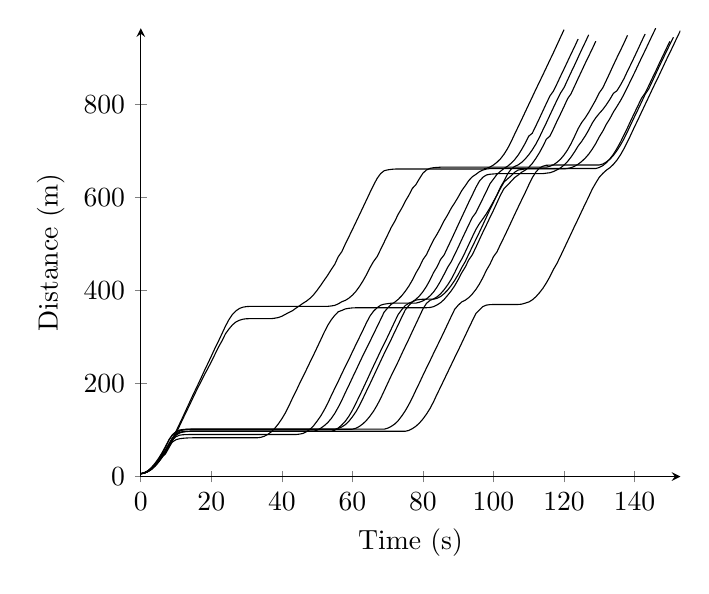
\begin{tikzpicture}
\begin{axis}[
legend style={anchor=west},
axis x line=bottom,
axis y line=left,
ymin=-1,
xlabel=Time (s),
ylabel=Distance (m),
]
\addplot[] coordinates {
(0, 5.1)
(1, 7.46923046061)
(2, 11.6173422848)
(3, 18.1501737379)
(4, 27.1587242881)
(5, 37.6107251469)
(6, 49.958897774)
(7, 63.7102691849)
(8, 78.632107588)
(9, 89.2214787016)
(10, 95.5532762341)
(11, 99.1027406392)
(12, 100.419624944)
(13, 101.006920344)
(14, 101.035490889)
(15, 101.035490889)
(16, 101.035490889)
(17, 101.035490889)
(18, 101.035490889)
(19, 101.035490889)
(20, 101.035490889)
(21, 101.035490889)
(22, 101.035490889)
(23, 101.035490889)
(24, 101.035490889)
(25, 101.035490889)
(26, 101.035490889)
(27, 101.035490889)
(28, 101.035490889)
(29, 101.035490889)
(30, 101.035490889)
(31, 101.035490889)
(32, 101.035490889)
(33, 101.035490889)
(34, 101.035490889)
(35, 101.035490889)
(36, 101.035490889)
(37, 101.035490889)
(38, 101.035490889)
(39, 101.035490889)
(40, 101.035490889)
(41, 101.035490889)
(42, 101.035490889)
(43, 101.035490889)
(44, 101.035490889)
(45, 101.035490889)
(46, 101.035490889)
(47, 101.035490889)
(48, 101.035490889)
(49, 101.035490889)
(50, 101.035490889)
(51, 101.035490889)
(52, 101.035490889)
(53, 101.035490889)
(54, 101.035490889)
(55, 101.035490889)
(56, 102.822179283)
(57, 105.888135585)
(58, 110.811076218)
(59, 118.063728433)
(60, 127.611864709)
(61, 138.548276489)
(62, 151.889088845)
(63, 167.40125684)
(64, 183.377397155)
(65, 198.97995483)
(66, 215.118117296)
(67, 231.367143516)
(68, 247.588162869)
(69, 263.728854296)
(70, 279.319354457)
(71, 294.453362918)
(72, 310.694681456)
(73, 326.14801551)
(74, 342.605639665)
(75, 358.052322929)
(76, 367.445762589)
(77, 375.328865871)
(78, 379.064217048)
(79, 380.490493206)
(80, 381.01477031)
(81, 381.081516622)
(82, 381.09846024)
(83, 381.10953119)
(84, 382.949669289)
(85, 386.76871709)
(86, 392.901113704)
(87, 400.701691383)
(88, 410.433622574)
(89, 421.550492008)
(90, 434.189078972)
(91, 449.073627901)
(92, 462.078264552)
(93, 478.393415343)
(94, 493.944893234)
(95, 509.688490598)
(96, 525.263101147)
(97, 541.445837832)
(98, 557.886342419)
(99, 574.317203868)
(100, 589.697069551)
(101, 606.046910557)
(102, 622.527630402)
(103, 635.786234196)
(104, 650.97983218)
(105, 661.036986101)
(106, 667.108889184)
(107, 670.43672285)
(108, 675.882500849)
(109, 683.23049228)
(110, 692.130342758)
(111, 702.772751202)
(112, 714.995439699)
(113, 729.442366742)
(114, 745.565911142)
(115, 761.209814625)
(116, 777.661244972)
(117, 793.845325634)
(118, 809.767737804)
(119, 825.199976352)
(120, 836.678116443)
(121, 853.234456705)
(122, 869.677300974)
(123, 885.502699798)
(124, 902.070323273)
(125, 918.520975071)
(126, 934.355071662)
(127, 950.707008784)
};
\addplot[] coordinates {
(0, 5.1)
(1, 6.55497497055)
(2, 9.50795923147)
(3, 13.983130693)
(4, 20.9410632881)
(5, 29.4022457877)
(6, 39.6907179732)
(7, 51.8153665074)
(8, 66.2571245323)
(9, 81.5171628758)
(10, 90.8626636902)
(11, 96.7088646274)
(12, 99.4614717735)
(13, 100.336197857)
(14, 100.75006219)
(15, 100.932266291)
(16, 101.016230257)
(17, 101.031113903)
(18, 101.031113903)
(19, 101.031113903)
(20, 101.031113903)
(21, 101.031113903)
(22, 101.031113903)
(23, 101.031113903)
(24, 101.031113903)
(25, 101.031113903)
(26, 101.031113903)
(27, 101.031113903)
(28, 101.031113903)
(29, 101.031113903)
(30, 101.031113903)
(31, 101.031113903)
(32, 101.031113903)
(33, 101.031113903)
(34, 101.031113903)
(35, 101.031113903)
(36, 101.031113903)
(37, 101.031113903)
(38, 101.031113903)
(39, 101.031113903)
(40, 101.031113903)
(41, 101.031113903)
(42, 101.031113903)
(43, 101.031113903)
(44, 101.031113903)
(45, 101.031113903)
(46, 101.031113903)
(47, 101.031113903)
(48, 101.031113903)
(49, 101.031113903)
(50, 101.031113903)
(51, 101.031113903)
(52, 101.031113903)
(53, 101.031113903)
(54, 101.031113903)
(55, 101.031113903)
(56, 101.031113903)
(57, 101.031113903)
(58, 101.031113903)
(59, 101.031113903)
(60, 101.031113903)
(61, 103.129192578)
(62, 107.097165717)
(63, 112.73578485)
(64, 120.095359602)
(65, 129.289343075)
(66, 139.862128061)
(67, 152.639672888)
(68, 167.247297722)
(69, 183.397790103)
(70, 199.83438427)
(71, 215.979568727)
(72, 231.330095053)
(73, 246.881657555)
(74, 263.433832387)
(75, 279.455655615)
(76, 295.161984846)
(77, 311.564750996)
(78, 327.717905623)
(79, 343.739815605)
(80, 360.119918035)
(81, 372.014727024)
(82, 378.586254246)
(83, 381.545842146)
(84, 386.138739913)
(85, 392.743453987)
(86, 401.389276046)
(87, 411.752547145)
(88, 423.741556894)
(89, 438.185223043)
(90, 454.07446782)
(91, 467.405973453)
(92, 482.770744646)
(93, 498.99090855)
(94, 515.284701683)
(95, 531.076678379)
(96, 543.696176245)
(97, 554.288429543)
(98, 565.314765361)
(99, 578.098225163)
(100, 591.731395025)
(101, 605.381950099)
(102, 620.143737008)
(103, 633.588393128)
(104, 640.396560268)
(105, 646.824176656)
(106, 654.55319761)
(107, 659.353228437)
(108, 660.504387314)
(109, 661.700675373)
(110, 661.780158821)
(111, 661.819719687)
(112, 661.819719687)
(113, 661.819719687)
(114, 661.819719687)
(115, 661.819719687)
(116, 661.819719687)
(117, 661.819719687)
(118, 661.819719687)
(119, 661.819719687)
(120, 661.819719687)
(121, 662.733796257)
(122, 664.417531421)
(123, 667.40165227)
(124, 671.884457431)
(125, 677.689511389)
(126, 684.895244372)
(127, 693.470532324)
(128, 704.248380546)
(129, 716.364709115)
(130, 730.798140728)
(131, 743.170580445)
(132, 757.908300549)
(133, 770.018589091)
(134, 784.252394017)
(135, 796.258664959)
(136, 808.63985779)
(137, 822.519968876)
(138, 837.921721814)
(139, 853.778720468)
(140, 869.184839915)
(141, 885.330852601)
(142, 901.466876091)
(143, 917.005462056)
(144, 933.073340988)
(145, 949.270876581)
(146, 964.814278837)
};
\addplot[] coordinates {
(0, 5.1)
(1, 6.67341325481)
(2, 10.7103693251)
(3, 16.3473940337)
(4, 24.3962265687)
(5, 34.8386510659)
(6, 46.5916361499)
(7, 56.2085086884)
(8, 70.10942799)
(9, 82.7041849737)
(10, 90.6931217674)
(11, 93.8543420516)
(12, 95.8768317498)
(13, 96.3857193463)
(14, 96.5273239925)
(15, 96.5726075927)
(16, 96.5859173751)
(17, 96.5859173751)
(18, 96.5859173751)
(19, 96.5859173751)
(20, 96.5859173751)
(21, 96.5859173751)
(22, 96.5859173751)
(23, 96.5859173751)
(24, 96.5859173751)
(25, 96.5859173751)
(26, 96.5859173751)
(27, 96.5859173751)
(28, 96.5859173751)
(29, 96.5859173751)
(30, 96.5859173751)
(31, 96.5859173751)
(32, 96.5859173751)
(33, 96.5859173751)
(34, 96.5859173751)
(35, 96.5859173751)
(36, 96.5859173751)
(37, 96.5859173751)
(38, 96.5859173751)
(39, 96.5859173751)
(40, 96.5859173751)
(41, 96.5859173751)
(42, 96.5859173751)
(43, 96.5859173751)
(44, 96.5859173751)
(45, 96.5859173751)
(46, 96.5859173751)
(47, 96.5859173751)
(48, 96.5859173751)
(49, 96.5859173751)
(50, 98.896801507)
(51, 102.992601833)
(52, 108.453662375)
(53, 115.203341681)
(54, 123.986467005)
(55, 135.016366098)
(56, 148.49814047)
(57, 163.328277239)
(58, 179.807507588)
(59, 195.425866425)
(60, 211.830039585)
(61, 227.64956941)
(62, 243.971944311)
(63, 259.984769635)
(64, 275.398984011)
(65, 290.41539293)
(66, 306.169609849)
(67, 321.635282244)
(68, 337.394349324)
(69, 353.191705238)
(70, 362.123311038)
(71, 370.059671182)
(72, 374.602819547)
(73, 380.831389743)
(74, 388.648487042)
(75, 398.196095263)
(76, 409.196961545)
(77, 422.163922801)
(78, 437.395310198)
(79, 450.175458285)
(80, 466.393383346)
(81, 477.005230762)
(82, 493.07970384)
(83, 508.54121178)
(84, 521.062045895)
(85, 534.909473416)
(86, 550.04540513)
(87, 562.601502146)
(88, 576.900104827)
(89, 588.608338255)
(90, 601.200516982)
(91, 614.928924082)
(92, 625.47799628)
(93, 636.729493421)
(94, 644.826074987)
(95, 649.959450767)
(96, 655.633342062)
(97, 659.309448063)
(98, 661.446610729)
(99, 662.417161786)
(100, 662.553028393)
(101, 662.553028393)
(102, 662.553028393)
(103, 662.553028393)
(104, 662.553028393)
(105, 662.553028393)
(106, 662.553028393)
(107, 662.553028393)
(108, 662.553028393)
(109, 662.553028393)
(110, 662.553028393)
(111, 662.553028393)
(112, 662.553028393)
(113, 662.553028393)
(114, 662.553028393)
(115, 662.553028393)
(116, 662.553028393)
(117, 662.553028393)
(118, 662.553028393)
(119, 662.553028393)
(120, 662.553028393)
(121, 662.553028393)
(122, 662.553028393)
(123, 662.553028393)
(124, 662.553028393)
(125, 662.553028393)
(126, 662.553028393)
(127, 662.553028393)
(128, 662.553028393)
(129, 662.553028393)
(130, 664.852251841)
(131, 668.886518499)
(132, 675.104247445)
(133, 683.322641856)
(134, 693.297545967)
(135, 705.68215057)
(136, 719.480531925)
(137, 734.920233521)
(138, 750.464510413)
(139, 766.875400738)
(140, 782.86415667)
(141, 798.627818291)
(142, 814.219567344)
(143, 825.207662155)
(144, 840.584734498)
(145, 856.800911462)
(146, 872.345188191)
(147, 888.864289687)
(148, 904.810411487)
(149, 920.72532611)
(150, 936.514357087)
};
\addplot[] coordinates {
(0, 5.1)
(1, 6.3517768683)
(2, 10.0052343078)
(3, 15.6389804591)
(4, 22.8560698093)
(5, 32.4239768736)
(6, 44.2262123155)
(7, 52.9564321958)
(8, 67.5881839456)
(9, 80.638561951)
(10, 88.894925948)
(11, 93.2029950287)
(12, 95.9533801613)
(13, 96.387872628)
(14, 96.4964753387)
(15, 96.5567803766)
(16, 96.5891625687)
(17, 96.5891625687)
(18, 96.5891625687)
(19, 96.5891625687)
(20, 96.5891625687)
(21, 96.5891625687)
(22, 96.5891625687)
(23, 96.5891625687)
(24, 96.5891625687)
(25, 96.5891625687)
(26, 96.5891625687)
(27, 96.5891625687)
(28, 96.5891625687)
(29, 96.5891625687)
(30, 96.5891625687)
(31, 96.5891625687)
(32, 96.5891625687)
(33, 96.5891625687)
(34, 96.5891625687)
(35, 96.5891625687)
(36, 96.5891625687)
(37, 96.5891625687)
(38, 96.5891625687)
(39, 96.5891625687)
(40, 96.5891625687)
(41, 96.5891625687)
(42, 96.5891625687)
(43, 96.5891625687)
(44, 96.5891625687)
(45, 96.5891625687)
(46, 96.5891625687)
(47, 96.5891625687)
(48, 96.5891625687)
(49, 96.5891625687)
(50, 96.5891625687)
(51, 96.5891625687)
(52, 96.5891625687)
(53, 96.5891625687)
(54, 96.5891625687)
(55, 96.5891625687)
(56, 96.5891625687)
(57, 96.5891625687)
(58, 96.5891625687)
(59, 96.5891625687)
(60, 96.5891625687)
(61, 96.5891625687)
(62, 96.5891625687)
(63, 96.5891625687)
(64, 96.5891625687)
(65, 96.5891625687)
(66, 96.5891625687)
(67, 96.5891625687)
(68, 96.5891625687)
(69, 96.5891625687)
(70, 96.5891625687)
(71, 96.5891625687)
(72, 96.5891625687)
(73, 96.5891625687)
(74, 96.5891625687)
(75, 96.5891625687)
(76, 98.3491453402)
(77, 102.15788792)
(78, 107.361901668)
(79, 114.238027927)
(80, 123.052356936)
(81, 133.45219528)
(82, 145.546490775)
(83, 160.013910662)
(84, 176.369042636)
(85, 191.817195209)
(86, 207.716465369)
(87, 223.549297283)
(88, 239.310363403)
(89, 255.237834505)
(90, 270.61824746)
(91, 286.634260235)
(92, 302.671686034)
(93, 318.837005337)
(94, 334.50544993)
(95, 350.042750605)
(96, 357.974055845)
(97, 365.163172689)
(98, 368.358050488)
(99, 369.383903031)
(100, 369.631448444)
(101, 369.703334999)
(102, 369.727885174)
(103, 369.727885174)
(104, 369.727885174)
(105, 369.727885174)
(106, 369.727885174)
(107, 369.727885174)
(108, 370.392086802)
(109, 372.636648368)
(110, 375.021786718)
(111, 379.526794264)
(112, 386.181693438)
(113, 394.637375123)
(114, 404.34975051)
(115, 416.231694545)
(116, 429.688913556)
(117, 445.192862866)
(118, 458.189740571)
(119, 473.811294415)
(120, 489.907779653)
(121, 506.010701487)
(122, 522.111864592)
(123, 538.381251425)
(124, 553.923194758)
(125, 570.322567085)
(126, 586.148888047)
(127, 601.817444525)
(128, 618.204363021)
(129, 631.36855419)
(130, 643.765951419)
(131, 652.057419245)
(132, 658.929836575)
(133, 664.394358764)
(134, 671.480312253)
(135, 680.645486147)
(136, 691.847264092)
(137, 705.424973406)
(138, 720.32279905)
(139, 736.188298033)
(140, 752.679758936)
(141, 768.236756988)
(142, 784.436532903)
(143, 800.544317406)
(144, 816.445683895)
(145, 832.715935547)
(146, 848.617247889)
(147, 864.077839866)
(148, 880.283292264)
(149, 896.565017747)
(150, 912.037707686)
(151, 927.791825213)
(152, 944.208865286)
(153, 959.595090993)
};
\addplot[] coordinates {
(0, 5.1)
(1, 6.80949328254)
(2, 10.7984346505)
(3, 17.1685230501)
(4, 25.6695144739)
(5, 35.6685858845)
(6, 47.858106465)
(7, 61.6694568597)
(8, 77.5137988256)
(9, 88.9991766891)
(10, 95.2163204122)
(11, 98.4340475669)
(12, 99.8789042802)
(13, 100.444085254)
(14, 100.838280779)
(15, 100.990214831)
(16, 101.016192608)
(17, 101.039551417)
(18, 101.039551417)
(19, 101.039551417)
(20, 101.039551417)
(21, 101.039551417)
(22, 101.039551417)
(23, 101.039551417)
(24, 101.039551417)
(25, 101.039551417)
(26, 101.039551417)
(27, 101.039551417)
(28, 101.039551417)
(29, 101.039551417)
(30, 101.039551417)
(31, 101.039551417)
(32, 101.039551417)
(33, 101.039551417)
(34, 101.039551417)
(35, 101.039551417)
(36, 101.039551417)
(37, 101.039551417)
(38, 101.039551417)
(39, 101.039551417)
(40, 101.039551417)
(41, 101.039551417)
(42, 101.039551417)
(43, 101.039551417)
(44, 101.039551417)
(45, 101.039551417)
(46, 101.039551417)
(47, 101.039551417)
(48, 101.039551417)
(49, 101.039551417)
(50, 101.039551417)
(51, 101.039551417)
(52, 101.039551417)
(53, 101.039551417)
(54, 101.039551417)
(55, 101.039551417)
(56, 101.039551417)
(57, 101.039551417)
(58, 101.039551417)
(59, 101.039551417)
(60, 101.039551417)
(61, 101.039551417)
(62, 101.039551417)
(63, 101.039551417)
(64, 101.039551417)
(65, 101.039551417)
(66, 101.039551417)
(67, 101.039551417)
(68, 101.039551417)
(69, 101.039551417)
(70, 103.223392604)
(71, 106.971201388)
(72, 112.115669793)
(73, 119.615278835)
(74, 129.512420014)
(75, 140.755917986)
(76, 154.103157576)
(77, 168.739134657)
(78, 185.040694261)
(79, 200.740014817)
(80, 217.033307838)
(81, 232.81640014)
(82, 248.263495951)
(83, 264.287267446)
(84, 279.815999099)
(85, 295.341151963)
(86, 311.238413248)
(87, 327.377783468)
(88, 343.497679821)
(89, 359.21949729)
(90, 368.072362198)
(91, 375.305026069)
(92, 378.920149009)
(93, 384.571524521)
(94, 392.347422723)
(95, 401.883459191)
(96, 413.618682504)
(97, 427.509878501)
(98, 443.44930495)
(99, 456.480601782)
(100, 472.678075504)
(101, 483.147807418)
(102, 499.410398744)
(103, 514.786708475)
(104, 530.718466287)
(105, 546.918311744)
(106, 563.372098955)
(107, 579.339642697)
(108, 595.153428439)
(109, 610.740242157)
(110, 627.111705539)
(111, 642.738482065)
(112, 654.726250826)
(113, 663.356797881)
(114, 667.560268009)
(115, 669.601792144)
(116, 669.929695821)
(117, 670.220794062)
(118, 670.252346783)
(119, 670.252346783)
(120, 670.252346783)
(121, 670.252346783)
(122, 670.252346783)
(123, 670.252346783)
(124, 670.252346783)
(125, 670.252346783)
(126, 670.252346783)
(127, 670.252346783)
(128, 670.252346783)
(129, 670.252346783)
(130, 670.252346783)
(131, 672.272553099)
(132, 676.614316431)
(133, 682.604135083)
(134, 690.8239749)
(135, 701.254130074)
(136, 712.991181577)
(137, 726.580362111)
(138, 742.125877807)
(139, 758.368172773)
(140, 774.48001693)
(141, 790.097068782)
(142, 806.038170846)
(143, 822.310486938)
(144, 833.669918217)
(145, 849.896447568)
(146, 866.302804332)
(147, 882.607058679)
(148, 898.419507633)
(149, 914.114216209)
(150, 929.717999632)
(151, 945.253470447)
};
\addplot[] coordinates {
(0, 5.1)
(1, 6.55653123996)
(2, 10.0533521605)
(3, 15.4822502031)
(4, 22.2821070343)
(5, 30.8229039905)
(6, 41.8539004947)
(7, 50.7660085335)
(8, 66.0878921338)
(9, 79.6948423047)
(10, 88.1784317213)
(11, 93.1071537926)
(12, 94.9371041241)
(13, 96.0054684435)
(14, 96.5416928404)
(15, 96.584277376)
(16, 96.584277376)
(17, 96.584277376)
(18, 96.584277376)
(19, 96.584277376)
(20, 96.584277376)
(21, 96.584277376)
(22, 96.584277376)
(23, 96.584277376)
(24, 96.584277376)
(25, 96.584277376)
(26, 96.584277376)
(27, 96.584277376)
(28, 96.584277376)
(29, 96.584277376)
(30, 96.584277376)
(31, 96.584277376)
(32, 96.584277376)
(33, 96.584277376)
(34, 96.584277376)
(35, 96.584277376)
(36, 96.584277376)
(37, 96.584277376)
(38, 96.584277376)
(39, 96.584277376)
(40, 96.584277376)
(41, 96.584277376)
(42, 96.584277376)
(43, 96.584277376)
(44, 96.584277376)
(45, 96.584277376)
(46, 96.584277376)
(47, 96.584277376)
(48, 96.584277376)
(49, 96.584277376)
(50, 96.584277376)
(51, 96.584277376)
(52, 96.584277376)
(53, 96.584277376)
(54, 96.584277376)
(55, 98.8997786332)
(56, 103.573816937)
(57, 110.160054119)
(58, 118.317360692)
(59, 128.867267329)
(60, 141.912422641)
(61, 157.042565883)
(62, 172.438829447)
(63, 188.418504537)
(64, 204.598317617)
(65, 221.093638447)
(66, 237.45394068)
(67, 253.391491708)
(68, 269.510468816)
(69, 284.803296877)
(70, 300.413421617)
(71, 316.532764169)
(72, 332.746544642)
(73, 348.391360363)
(74, 358.585649492)
(75, 367.394486538)
(76, 372.444541138)
(77, 375.555469016)
(78, 380.808783103)
(79, 388.017196918)
(80, 397.262132571)
(81, 408.731349492)
(82, 422.493818649)
(83, 438.226738383)
(84, 450.696283648)
(85, 466.644114447)
(86, 476.347161745)
(87, 492.603839381)
(88, 508.420951429)
(89, 524.862808536)
(90, 541.295428198)
(91, 557.657520855)
(92, 573.819821357)
(93, 590.168753878)
(94, 605.642885181)
(95, 621.610764551)
(96, 635.351244978)
(97, 643.741948964)
(98, 648.655925788)
(99, 650.219077889)
(100, 650.864324753)
(101, 651.421306609)
(102, 651.512579756)
(103, 651.541946322)
(104, 651.553311652)
(105, 651.553311652)
(106, 651.553311652)
(107, 651.553311652)
(108, 651.553311652)
(109, 651.553311652)
(110, 651.553311652)
(111, 651.553311652)
(112, 651.553311652)
(113, 651.553311652)
(114, 651.553311652)
(115, 652.599340484)
(116, 653.466234996)
(117, 656.05399213)
(118, 659.626444936)
(119, 663.911420674)
(120, 670.123770155)
(121, 677.618253899)
(122, 687.306707377)
(123, 698.489657561)
(124, 711.0149283)
(125, 721.004800412)
(126, 732.482828906)
(127, 745.534125388)
(128, 760.460713285)
(129, 771.887250511)
(130, 781.251339613)
(131, 789.777498191)
(132, 799.993921576)
(133, 811.56350051)
(134, 824.498884603)
(135, 830.09653038)
(136, 842.353995102)
(137, 856.199087541)
(138, 872.468355312)
(139, 887.961688073)
(140, 903.857530706)
(141, 920.006305147)
(142, 936.548651356)
(143, 952.297994243)
};
\addplot[] coordinates {
(0, 5.1)
(1, 6.44659333242)
(2, 9.8037742642)
(3, 15.3562089049)
(4, 22.7431525589)
(5, 31.6042632478)
(6, 41.7737365432)
(7, 49.8019061767)
(8, 64.4532271425)
(9, 73.627579412)
(10, 78.4570317695)
(11, 80.4580726328)
(12, 81.4543018877)
(13, 82.0798181715)
(14, 82.4064942339)
(15, 82.5468847082)
(16, 82.56624516)
(17, 82.5816362954)
(18, 82.5816362954)
(19, 82.5816362954)
(20, 82.5816362954)
(21, 82.5816362954)
(22, 82.5816362954)
(23, 82.5816362954)
(24, 82.5816362954)
(25, 82.5816362954)
(26, 82.5816362954)
(27, 82.5816362954)
(28, 82.5816362954)
(29, 82.5816362954)
(30, 82.5816362954)
(31, 82.5816362954)
(32, 82.5816362954)
(33, 82.5816362954)
(34, 83.4173252922)
(35, 85.7716148228)
(36, 89.6830617939)
(37, 95.3472956129)
(38, 102.978381468)
(39, 112.402909046)
(40, 123.423779665)
(41, 136.113098524)
(42, 151.255150835)
(43, 167.562310759)
(44, 182.749282906)
(45, 199.000918673)
(46, 214.111123822)
(47, 229.823063838)
(48, 245.644767473)
(49, 261.108498768)
(50, 277.181726276)
(51, 293.205187887)
(52, 309.593964339)
(53, 324.566651482)
(54, 336.575299073)
(55, 346.346652994)
(56, 354.064477134)
(57, 356.832432186)
(58, 360.167655346)
(59, 361.495640557)
(60, 362.273446151)
(61, 362.621960203)
(62, 362.694777648)
(63, 362.717839806)
(64, 362.724812917)
(65, 362.724812917)
(66, 362.724812917)
(67, 362.724812917)
(68, 362.724812917)
(69, 362.724812917)
(70, 362.724812917)
(71, 362.724812917)
(72, 362.724812917)
(73, 362.724812917)
(74, 362.724812917)
(75, 362.724812917)
(76, 362.724812917)
(77, 362.724812917)
(78, 362.724812917)
(79, 362.724812917)
(80, 362.724812917)
(81, 362.724812917)
(82, 363.202074481)
(83, 365.012124073)
(84, 368.728664547)
(85, 373.526613937)
(86, 380.459384992)
(87, 389.485199147)
(88, 398.887303176)
(89, 409.960654982)
(90, 423.283771006)
(91, 437.939901301)
(92, 450.335562194)
(93, 465.835220494)
(94, 476.736429136)
(95, 492.605559445)
(96, 509.163048215)
(97, 525.452929104)
(98, 541.068953761)
(99, 557.114582396)
(100, 572.58186831)
(101, 589.083239497)
(102, 605.591469679)
(103, 619.535009458)
(104, 626.825053488)
(105, 635.025707111)
(106, 643.140809683)
(107, 648.564670343)
(108, 654.627288857)
(109, 659.003940004)
(110, 665.082134716)
(111, 673.446279128)
(112, 684.20528917)
(113, 696.358500031)
(114, 710.299731818)
(115, 725.751128548)
(116, 732.336626628)
(117, 747.99917949)
(118, 764.48943536)
(119, 779.968309965)
(120, 796.108127225)
(121, 812.609558846)
(122, 823.81237011)
(123, 840.127861333)
(124, 856.60640032)
(125, 872.678621131)
(126, 889.063489218)
(127, 904.670122654)
(128, 920.269251725)
(129, 936.778072217)
};
\addplot[] coordinates {
(0, 5.1)
(1, 6.73179594907)
(2, 9.69965092421)
(3, 15.1289977976)
(4, 22.8809571521)
(5, 32.9460635696)
(6, 45.2490242858)
(7, 55.1510169741)
(8, 67.2376854506)
(9, 78.2903558592)
(10, 84.8795739575)
(11, 88.1323106067)
(12, 89.1149851304)
(13, 89.3982309467)
(14, 89.5792341189)
(15, 89.5884724929)
(16, 89.5884724929)
(17, 89.5884724929)
(18, 89.5884724929)
(19, 89.5884724929)
(20, 89.5884724929)
(21, 89.5884724929)
(22, 89.5884724929)
(23, 89.5884724929)
(24, 89.5884724929)
(25, 89.5884724929)
(26, 89.5884724929)
(27, 89.5884724929)
(28, 89.5884724929)
(29, 89.5884724929)
(30, 89.5884724929)
(31, 89.5884724929)
(32, 89.5884724929)
(33, 89.5884724929)
(34, 89.5884724929)
(35, 89.5884724929)
(36, 89.5884724929)
(37, 89.5884724929)
(38, 89.5884724929)
(39, 89.5884724929)
(40, 89.5884724929)
(41, 89.5884724929)
(42, 89.5884724929)
(43, 89.5884724929)
(44, 89.5884724929)
(45, 90.3782250109)
(46, 91.9395265799)
(47, 95.8212367189)
(48, 101.011654294)
(49, 108.506383915)
(50, 118.45452067)
(51, 129.15853527)
(52, 142.158406429)
(53, 156.698697443)
(54, 173.112367601)
(55, 188.916367648)
(56, 204.291346435)
(57, 220.552757715)
(58, 236.211018901)
(59, 251.249455263)
(60, 267.598290963)
(61, 283.324102124)
(62, 298.857461341)
(63, 314.458836797)
(64, 330.635630587)
(65, 344.947461056)
(66, 355.327918305)
(67, 362.572886708)
(68, 368.148769417)
(69, 370.409969645)
(70, 371.502024339)
(71, 372.452873588)
(72, 372.606309603)
(73, 372.641840834)
(74, 372.652675739)
(75, 372.652675739)
(76, 372.652675739)
(77, 372.652675739)
(78, 372.652675739)
(79, 374.582244884)
(80, 377.492595705)
(81, 381.683326016)
(82, 388.171903484)
(83, 396.487647144)
(84, 407.279294434)
(85, 420.230761081)
(86, 434.656708191)
(87, 449.667748844)
(88, 461.595203801)
(89, 477.322339134)
(90, 492.930978502)
(91, 509.441548279)
(92, 525.647602359)
(93, 541.408410423)
(94, 557.274558057)
(95, 567.197960323)
(96, 582.534565167)
(97, 598.073108264)
(98, 613.539637925)
(99, 629.624384741)
(100, 639.847025147)
(101, 650.136926495)
(102, 656.617432642)
(103, 662.912611908)
(104, 667.542304945)
(105, 673.88378254)
(106, 681.675371159)
(107, 691.494930741)
(108, 703.627579588)
(109, 717.08107434)
(110, 732.249829739)
(111, 738.595553412)
(112, 754.21203147)
(113, 770.143991986)
(114, 786.630733659)
(115, 802.883213277)
(116, 818.879627002)
(117, 829.445365634)
(118, 845.024331757)
(119, 861.235541745)
(120, 877.067858037)
(121, 893.239148443)
(122, 909.322307259)
(123, 925.083958804)
(124, 941.591845322)
};
\addplot[] coordinates {
(0, 5.1)
(1, 6.86160143077)
(2, 10.4317740693)
(3, 15.4916550035)
(4, 21.8200966054)
(5, 30.3460729962)
(6, 40.678570478)
(7, 47.9870070575)
(8, 61.1587519425)
(9, 75.6332798136)
(10, 92.2162075416)
(11, 108.178216636)
(12, 124.35168552)
(13, 139.952921119)
(14, 155.747547525)
(15, 171.822303203)
(16, 187.71788651)
(17, 202.318742309)
(18, 217.755422192)
(19, 231.565259786)
(20, 246.318391898)
(21, 261.765089657)
(22, 277.306284248)
(23, 290.943396934)
(24, 306.310235615)
(25, 316.868052441)
(26, 325.768084806)
(27, 332.223370267)
(28, 335.781984032)
(29, 338.045900409)
(30, 338.994324321)
(31, 339.151197504)
(32, 339.165591291)
(33, 339.172536584)
(34, 339.172536584)
(35, 339.172536584)
(36, 339.172536584)
(37, 339.172536584)
(38, 340.170598621)
(39, 341.52007607)
(40, 344.352392621)
(41, 348.425692444)
(42, 352.581826273)
(43, 356.200908927)
(44, 361.876458631)
(45, 366.855494775)
(46, 372.310706505)
(47, 376.991257477)
(48, 383.104552484)
(49, 390.728380553)
(50, 400.243699809)
(51, 410.795041872)
(52, 421.872404711)
(53, 432.732563567)
(54, 444.950105255)
(55, 456.189991757)
(56, 472.7011653)
(57, 483.453227192)
(58, 500.00716847)
(59, 515.474011747)
(60, 530.978243418)
(61, 546.957027638)
(62, 562.893925124)
(63, 578.887113429)
(64, 594.929375205)
(65, 611.131104537)
(66, 626.741390237)
(67, 641.129200285)
(68, 651.626982872)
(69, 657.754513466)
(70, 659.673765146)
(71, 660.769690376)
(72, 661.413907751)
(73, 661.522636564)
(74, 661.58155266)
(75, 661.631561475)
(76, 661.631561475)
(77, 661.631561475)
(78, 661.631561475)
(79, 661.631561475)
(80, 661.631561475)
(81, 661.631561475)
(82, 661.631561475)
(83, 661.631561475)
(84, 661.631561475)
(85, 661.631561475)
(86, 661.631561475)
(87, 661.631561475)
(88, 661.631561475)
(89, 661.631561475)
(90, 661.631561475)
(91, 661.631561475)
(92, 661.631561475)
(93, 661.631561475)
(94, 661.631561475)
(95, 661.631561475)
(96, 661.631561475)
(97, 661.631561475)
(98, 662.876523533)
(99, 665.748596593)
(100, 670.154872568)
(101, 676.12730741)
(102, 683.579351112)
(103, 693.48081515)
(104, 705.678550985)
(105, 720.242189182)
(106, 736.598080341)
(107, 752.325957317)
(108, 768.285860929)
(109, 784.398338946)
(110, 800.566840453)
(111, 816.5785702)
(112, 832.832357012)
(113, 848.486486414)
(114, 864.261619309)
(115, 880.226154425)
(116, 896.343650258)
(117, 912.15772197)
(118, 928.746842015)
(119, 945.217652884)
(120, 961.649558953)
};
\addplot[] coordinates {
(0, 5.1)
(1, 6.70178072576)
(2, 9.68408416831)
(3, 14.5174219514)
(4, 21.5369454063)
(5, 31.0560408973)
(6, 42.0466863718)
(7, 50.458786556)
(8, 64.8176235522)
(9, 80.8375829315)
(10, 96.5757364069)
(11, 112.451822349)
(12, 128.529371763)
(13, 145.084275352)
(14, 161.550936313)
(15, 178.008959092)
(16, 193.607007683)
(17, 209.900025428)
(18, 226.427428126)
(19, 242.252602544)
(20, 258.391110316)
(21, 274.863323617)
(22, 290.20719004)
(23, 306.448365096)
(24, 322.767038853)
(25, 337.037702367)
(26, 348.406102574)
(27, 356.03300944)
(28, 361.203550407)
(29, 363.96486972)
(30, 365.15841)
(31, 365.614036147)
(32, 365.640388947)
(33, 365.654405798)
(34, 365.654405798)
(35, 365.654405798)
(36, 365.654405798)
(37, 365.654405798)
(38, 365.654405798)
(39, 365.654405798)
(40, 365.654405798)
(41, 365.654405798)
(42, 365.654405798)
(43, 365.654405798)
(44, 365.654405798)
(45, 365.654405798)
(46, 365.654405798)
(47, 365.654405798)
(48, 365.654405798)
(49, 365.654405798)
(50, 365.654405798)
(51, 365.654405798)
(52, 365.654405798)
(53, 365.654405798)
(54, 366.500112252)
(55, 367.822392335)
(56, 371.004371521)
(57, 375.65086423)
(58, 378.477303661)
(59, 383.275137962)
(60, 389.721434796)
(61, 397.985699663)
(62, 408.382934901)
(63, 420.468063166)
(64, 433.940798964)
(65, 449.099445377)
(66, 462.382192874)
(67, 472.687334136)
(68, 488.136301709)
(69, 503.762125272)
(70, 519.476295562)
(71, 535.457338445)
(72, 548.628160279)
(73, 564.277888556)
(74, 577.122014315)
(75, 592.111817122)
(76, 604.858708232)
(77, 619.670564064)
(78, 627.844832142)
(79, 640.697958031)
(80, 652.551005892)
(81, 659.414405618)
(82, 662.960872562)
(83, 664.370807021)
(84, 664.931849786)
(85, 665.455273805)
(86, 665.520702813)
(87, 665.550667348)
(88, 665.550667348)
(89, 665.550667348)
(90, 665.550667348)
(91, 665.550667348)
(92, 665.550667348)
(93, 665.550667348)
(94, 665.550667348)
(95, 665.550667348)
(96, 665.550667348)
(97, 665.550667348)
(98, 665.550667348)
(99, 665.550667348)
(100, 665.550667348)
(101, 665.550667348)
(102, 665.550667348)
(103, 665.550667348)
(104, 665.550667348)
(105, 665.550667348)
(106, 665.550667348)
(107, 665.550667348)
(108, 665.550667348)
(109, 665.550667348)
(110, 665.550667348)
(111, 665.550667348)
(112, 665.550667348)
(113, 665.550667348)
(114, 665.550667348)
(115, 665.550667348)
(116, 667.411212649)
(117, 670.527756514)
(118, 675.877497828)
(119, 682.548572186)
(120, 691.610592673)
(121, 702.774126692)
(122, 716.165165431)
(123, 731.963237688)
(124, 748.370975174)
(125, 761.599483532)
(126, 771.611899367)
(127, 783.526849298)
(128, 796.92386057)
(129, 810.361426451)
(130, 825.789533583)
(131, 836.428021248)
(132, 852.55973391)
(133, 868.774329722)
(134, 885.33507909)
(135, 901.438575225)
(136, 916.805813402)
(137, 932.913497886)
(138, 949.443332482)
};

\end{axis}
\end{tikzpicture}
\label{tik:distance:0:51}
\caption{0 percent diving with GSC on route $51$}
\end{figure}

%
\begin{figure}
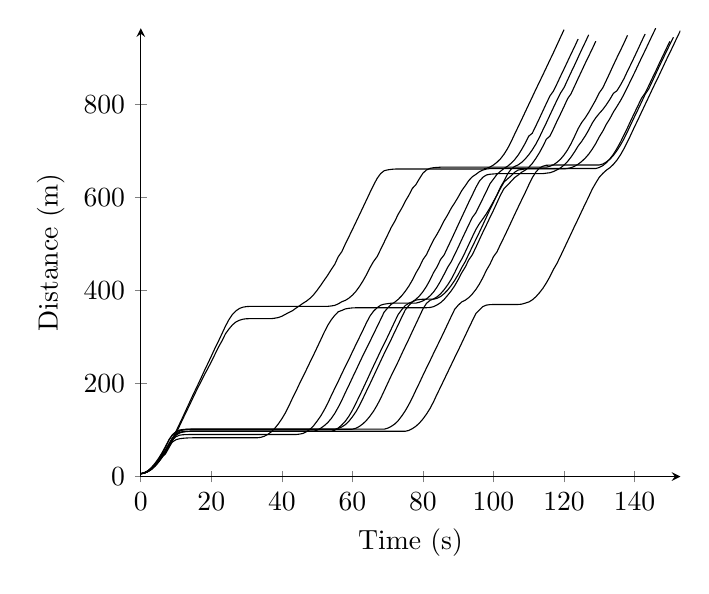
\begin{tikzpicture}
\begin{axis}[
legend style={anchor=west},
axis x line=bottom,
axis y line=left,
ymin=-1,
xlabel=Time (s),
ylabel=Distance (m),
]
\addplot[] coordinates {
(0, 5.1)
(1, 7.46923046061)
(2, 11.6173422848)
(3, 18.1501737379)
(4, 27.1587242881)
(5, 37.6107251469)
(6, 49.958897774)
(7, 63.7102691849)
(8, 78.632107588)
(9, 89.2214787016)
(10, 95.5532762341)
(11, 99.1027406392)
(12, 100.419624944)
(13, 101.006920344)
(14, 101.035490889)
(15, 101.035490889)
(16, 101.035490889)
(17, 101.035490889)
(18, 101.035490889)
(19, 101.035490889)
(20, 101.035490889)
(21, 101.035490889)
(22, 101.035490889)
(23, 101.035490889)
(24, 101.035490889)
(25, 101.035490889)
(26, 101.035490889)
(27, 101.035490889)
(28, 101.035490889)
(29, 101.035490889)
(30, 101.035490889)
(31, 101.035490889)
(32, 101.035490889)
(33, 101.035490889)
(34, 101.035490889)
(35, 101.035490889)
(36, 101.035490889)
(37, 101.035490889)
(38, 101.035490889)
(39, 101.035490889)
(40, 101.035490889)
(41, 101.035490889)
(42, 101.035490889)
(43, 101.035490889)
(44, 101.035490889)
(45, 101.035490889)
(46, 101.035490889)
(47, 101.035490889)
(48, 101.035490889)
(49, 101.035490889)
(50, 101.035490889)
(51, 101.035490889)
(52, 101.035490889)
(53, 101.035490889)
(54, 101.035490889)
(55, 101.035490889)
(56, 102.822179283)
(57, 105.888135585)
(58, 110.811076218)
(59, 118.063728433)
(60, 127.611864709)
(61, 138.548276489)
(62, 151.889088845)
(63, 167.40125684)
(64, 183.377397155)
(65, 198.97995483)
(66, 215.118117296)
(67, 231.367143516)
(68, 247.588162869)
(69, 263.728854296)
(70, 279.319354457)
(71, 294.453362918)
(72, 310.694681456)
(73, 326.14801551)
(74, 342.605639665)
(75, 358.052322929)
(76, 367.445762589)
(77, 375.328865871)
(78, 379.064217048)
(79, 380.490493206)
(80, 381.01477031)
(81, 381.081516622)
(82, 381.09846024)
(83, 381.10953119)
(84, 382.949669289)
(85, 386.76871709)
(86, 392.901113704)
(87, 400.701691383)
(88, 410.433622574)
(89, 421.550492008)
(90, 434.189078972)
(91, 449.073627901)
(92, 462.078264552)
(93, 478.393415343)
(94, 493.944893234)
(95, 509.688490598)
(96, 525.263101147)
(97, 541.445837832)
(98, 557.886342419)
(99, 574.317203868)
(100, 589.697069551)
(101, 606.046910557)
(102, 622.527630402)
(103, 635.786234196)
(104, 650.97983218)
(105, 661.036986101)
(106, 667.108889184)
(107, 670.43672285)
(108, 675.882500849)
(109, 683.23049228)
(110, 692.130342758)
(111, 702.772751202)
(112, 714.995439699)
(113, 729.442366742)
(114, 745.565911142)
(115, 761.209814625)
(116, 777.661244972)
(117, 793.845325634)
(118, 809.767737804)
(119, 825.199976352)
(120, 836.678116443)
(121, 853.234456705)
(122, 869.677300974)
(123, 885.502699798)
(124, 902.070323273)
(125, 918.520975071)
(126, 934.355071662)
(127, 950.707008784)
};
\addplot[] coordinates {
(0, 5.1)
(1, 6.55497497055)
(2, 9.50795923147)
(3, 13.983130693)
(4, 20.9410632881)
(5, 29.4022457877)
(6, 39.6907179732)
(7, 51.8153665074)
(8, 66.2571245323)
(9, 81.5171628758)
(10, 90.8626636902)
(11, 96.7088646274)
(12, 99.4614717735)
(13, 100.336197857)
(14, 100.75006219)
(15, 100.932266291)
(16, 101.016230257)
(17, 101.031113903)
(18, 101.031113903)
(19, 101.031113903)
(20, 101.031113903)
(21, 101.031113903)
(22, 101.031113903)
(23, 101.031113903)
(24, 101.031113903)
(25, 101.031113903)
(26, 101.031113903)
(27, 101.031113903)
(28, 101.031113903)
(29, 101.031113903)
(30, 101.031113903)
(31, 101.031113903)
(32, 101.031113903)
(33, 101.031113903)
(34, 101.031113903)
(35, 101.031113903)
(36, 101.031113903)
(37, 101.031113903)
(38, 101.031113903)
(39, 101.031113903)
(40, 101.031113903)
(41, 101.031113903)
(42, 101.031113903)
(43, 101.031113903)
(44, 101.031113903)
(45, 101.031113903)
(46, 101.031113903)
(47, 101.031113903)
(48, 101.031113903)
(49, 101.031113903)
(50, 101.031113903)
(51, 101.031113903)
(52, 101.031113903)
(53, 101.031113903)
(54, 101.031113903)
(55, 101.031113903)
(56, 101.031113903)
(57, 101.031113903)
(58, 101.031113903)
(59, 101.031113903)
(60, 101.031113903)
(61, 103.129192578)
(62, 107.097165717)
(63, 112.73578485)
(64, 120.095359602)
(65, 129.289343075)
(66, 139.862128061)
(67, 152.639672888)
(68, 167.247297722)
(69, 183.397790103)
(70, 199.83438427)
(71, 215.979568727)
(72, 231.330095053)
(73, 246.881657555)
(74, 263.433832387)
(75, 279.455655615)
(76, 295.161984846)
(77, 311.564750996)
(78, 327.717905623)
(79, 343.739815605)
(80, 360.119918035)
(81, 372.014727024)
(82, 378.586254246)
(83, 381.545842146)
(84, 386.138739913)
(85, 392.743453987)
(86, 401.389276046)
(87, 411.752547145)
(88, 423.741556894)
(89, 438.185223043)
(90, 454.07446782)
(91, 467.405973453)
(92, 482.770744646)
(93, 498.99090855)
(94, 515.284701683)
(95, 531.076678379)
(96, 543.696176245)
(97, 554.288429543)
(98, 565.314765361)
(99, 578.098225163)
(100, 591.731395025)
(101, 605.381950099)
(102, 620.143737008)
(103, 633.588393128)
(104, 640.396560268)
(105, 646.824176656)
(106, 654.55319761)
(107, 659.353228437)
(108, 660.504387314)
(109, 661.700675373)
(110, 661.780158821)
(111, 661.819719687)
(112, 661.819719687)
(113, 661.819719687)
(114, 661.819719687)
(115, 661.819719687)
(116, 661.819719687)
(117, 661.819719687)
(118, 661.819719687)
(119, 661.819719687)
(120, 661.819719687)
(121, 662.733796257)
(122, 664.417531421)
(123, 667.40165227)
(124, 671.884457431)
(125, 677.689511389)
(126, 684.895244372)
(127, 693.470532324)
(128, 704.248380546)
(129, 716.364709115)
(130, 730.798140728)
(131, 743.170580445)
(132, 757.908300549)
(133, 770.018589091)
(134, 784.252394017)
(135, 796.258664959)
(136, 808.63985779)
(137, 822.519968876)
(138, 837.921721814)
(139, 853.778720468)
(140, 869.184839915)
(141, 885.330852601)
(142, 901.466876091)
(143, 917.005462056)
(144, 933.073340988)
(145, 949.270876581)
(146, 964.814278837)
};
\addplot[] coordinates {
(0, 5.1)
(1, 6.67341325481)
(2, 10.7103693251)
(3, 16.3473940337)
(4, 24.3962265687)
(5, 34.8386510659)
(6, 46.5916361499)
(7, 56.2085086884)
(8, 70.10942799)
(9, 82.7041849737)
(10, 90.6931217674)
(11, 93.8543420516)
(12, 95.8768317498)
(13, 96.3857193463)
(14, 96.5273239925)
(15, 96.5726075927)
(16, 96.5859173751)
(17, 96.5859173751)
(18, 96.5859173751)
(19, 96.5859173751)
(20, 96.5859173751)
(21, 96.5859173751)
(22, 96.5859173751)
(23, 96.5859173751)
(24, 96.5859173751)
(25, 96.5859173751)
(26, 96.5859173751)
(27, 96.5859173751)
(28, 96.5859173751)
(29, 96.5859173751)
(30, 96.5859173751)
(31, 96.5859173751)
(32, 96.5859173751)
(33, 96.5859173751)
(34, 96.5859173751)
(35, 96.5859173751)
(36, 96.5859173751)
(37, 96.5859173751)
(38, 96.5859173751)
(39, 96.5859173751)
(40, 96.5859173751)
(41, 96.5859173751)
(42, 96.5859173751)
(43, 96.5859173751)
(44, 96.5859173751)
(45, 96.5859173751)
(46, 96.5859173751)
(47, 96.5859173751)
(48, 96.5859173751)
(49, 96.5859173751)
(50, 98.896801507)
(51, 102.992601833)
(52, 108.453662375)
(53, 115.203341681)
(54, 123.986467005)
(55, 135.016366098)
(56, 148.49814047)
(57, 163.328277239)
(58, 179.807507588)
(59, 195.425866425)
(60, 211.830039585)
(61, 227.64956941)
(62, 243.971944311)
(63, 259.984769635)
(64, 275.398984011)
(65, 290.41539293)
(66, 306.169609849)
(67, 321.635282244)
(68, 337.394349324)
(69, 353.191705238)
(70, 362.123311038)
(71, 370.059671182)
(72, 374.602819547)
(73, 380.831389743)
(74, 388.648487042)
(75, 398.196095263)
(76, 409.196961545)
(77, 422.163922801)
(78, 437.395310198)
(79, 450.175458285)
(80, 466.393383346)
(81, 477.005230762)
(82, 493.07970384)
(83, 508.54121178)
(84, 521.062045895)
(85, 534.909473416)
(86, 550.04540513)
(87, 562.601502146)
(88, 576.900104827)
(89, 588.608338255)
(90, 601.200516982)
(91, 614.928924082)
(92, 625.47799628)
(93, 636.729493421)
(94, 644.826074987)
(95, 649.959450767)
(96, 655.633342062)
(97, 659.309448063)
(98, 661.446610729)
(99, 662.417161786)
(100, 662.553028393)
(101, 662.553028393)
(102, 662.553028393)
(103, 662.553028393)
(104, 662.553028393)
(105, 662.553028393)
(106, 662.553028393)
(107, 662.553028393)
(108, 662.553028393)
(109, 662.553028393)
(110, 662.553028393)
(111, 662.553028393)
(112, 662.553028393)
(113, 662.553028393)
(114, 662.553028393)
(115, 662.553028393)
(116, 662.553028393)
(117, 662.553028393)
(118, 662.553028393)
(119, 662.553028393)
(120, 662.553028393)
(121, 662.553028393)
(122, 662.553028393)
(123, 662.553028393)
(124, 662.553028393)
(125, 662.553028393)
(126, 662.553028393)
(127, 662.553028393)
(128, 662.553028393)
(129, 662.553028393)
(130, 664.852251841)
(131, 668.886518499)
(132, 675.104247445)
(133, 683.322641856)
(134, 693.297545967)
(135, 705.68215057)
(136, 719.480531925)
(137, 734.920233521)
(138, 750.464510413)
(139, 766.875400738)
(140, 782.86415667)
(141, 798.627818291)
(142, 814.219567344)
(143, 825.207662155)
(144, 840.584734498)
(145, 856.800911462)
(146, 872.345188191)
(147, 888.864289687)
(148, 904.810411487)
(149, 920.72532611)
(150, 936.514357087)
};
\addplot[] coordinates {
(0, 5.1)
(1, 6.3517768683)
(2, 10.0052343078)
(3, 15.6389804591)
(4, 22.8560698093)
(5, 32.4239768736)
(6, 44.2262123155)
(7, 52.9564321958)
(8, 67.5881839456)
(9, 80.638561951)
(10, 88.894925948)
(11, 93.2029950287)
(12, 95.9533801613)
(13, 96.387872628)
(14, 96.4964753387)
(15, 96.5567803766)
(16, 96.5891625687)
(17, 96.5891625687)
(18, 96.5891625687)
(19, 96.5891625687)
(20, 96.5891625687)
(21, 96.5891625687)
(22, 96.5891625687)
(23, 96.5891625687)
(24, 96.5891625687)
(25, 96.5891625687)
(26, 96.5891625687)
(27, 96.5891625687)
(28, 96.5891625687)
(29, 96.5891625687)
(30, 96.5891625687)
(31, 96.5891625687)
(32, 96.5891625687)
(33, 96.5891625687)
(34, 96.5891625687)
(35, 96.5891625687)
(36, 96.5891625687)
(37, 96.5891625687)
(38, 96.5891625687)
(39, 96.5891625687)
(40, 96.5891625687)
(41, 96.5891625687)
(42, 96.5891625687)
(43, 96.5891625687)
(44, 96.5891625687)
(45, 96.5891625687)
(46, 96.5891625687)
(47, 96.5891625687)
(48, 96.5891625687)
(49, 96.5891625687)
(50, 96.5891625687)
(51, 96.5891625687)
(52, 96.5891625687)
(53, 96.5891625687)
(54, 96.5891625687)
(55, 96.5891625687)
(56, 96.5891625687)
(57, 96.5891625687)
(58, 96.5891625687)
(59, 96.5891625687)
(60, 96.5891625687)
(61, 96.5891625687)
(62, 96.5891625687)
(63, 96.5891625687)
(64, 96.5891625687)
(65, 96.5891625687)
(66, 96.5891625687)
(67, 96.5891625687)
(68, 96.5891625687)
(69, 96.5891625687)
(70, 96.5891625687)
(71, 96.5891625687)
(72, 96.5891625687)
(73, 96.5891625687)
(74, 96.5891625687)
(75, 96.5891625687)
(76, 98.3491453402)
(77, 102.15788792)
(78, 107.361901668)
(79, 114.238027927)
(80, 123.052356936)
(81, 133.45219528)
(82, 145.546490775)
(83, 160.013910662)
(84, 176.369042636)
(85, 191.817195209)
(86, 207.716465369)
(87, 223.549297283)
(88, 239.310363403)
(89, 255.237834505)
(90, 270.61824746)
(91, 286.634260235)
(92, 302.671686034)
(93, 318.837005337)
(94, 334.50544993)
(95, 350.042750605)
(96, 357.974055845)
(97, 365.163172689)
(98, 368.358050488)
(99, 369.383903031)
(100, 369.631448444)
(101, 369.703334999)
(102, 369.727885174)
(103, 369.727885174)
(104, 369.727885174)
(105, 369.727885174)
(106, 369.727885174)
(107, 369.727885174)
(108, 370.392086802)
(109, 372.636648368)
(110, 375.021786718)
(111, 379.526794264)
(112, 386.181693438)
(113, 394.637375123)
(114, 404.34975051)
(115, 416.231694545)
(116, 429.688913556)
(117, 445.192862866)
(118, 458.189740571)
(119, 473.811294415)
(120, 489.907779653)
(121, 506.010701487)
(122, 522.111864592)
(123, 538.381251425)
(124, 553.923194758)
(125, 570.322567085)
(126, 586.148888047)
(127, 601.817444525)
(128, 618.204363021)
(129, 631.36855419)
(130, 643.765951419)
(131, 652.057419245)
(132, 658.929836575)
(133, 664.394358764)
(134, 671.480312253)
(135, 680.645486147)
(136, 691.847264092)
(137, 705.424973406)
(138, 720.32279905)
(139, 736.188298033)
(140, 752.679758936)
(141, 768.236756988)
(142, 784.436532903)
(143, 800.544317406)
(144, 816.445683895)
(145, 832.715935547)
(146, 848.617247889)
(147, 864.077839866)
(148, 880.283292264)
(149, 896.565017747)
(150, 912.037707686)
(151, 927.791825213)
(152, 944.208865286)
(153, 959.595090993)
};
\addplot[] coordinates {
(0, 5.1)
(1, 6.80949328254)
(2, 10.7984346505)
(3, 17.1685230501)
(4, 25.6695144739)
(5, 35.6685858845)
(6, 47.858106465)
(7, 61.6694568597)
(8, 77.5137988256)
(9, 88.9991766891)
(10, 95.2163204122)
(11, 98.4340475669)
(12, 99.8789042802)
(13, 100.444085254)
(14, 100.838280779)
(15, 100.990214831)
(16, 101.016192608)
(17, 101.039551417)
(18, 101.039551417)
(19, 101.039551417)
(20, 101.039551417)
(21, 101.039551417)
(22, 101.039551417)
(23, 101.039551417)
(24, 101.039551417)
(25, 101.039551417)
(26, 101.039551417)
(27, 101.039551417)
(28, 101.039551417)
(29, 101.039551417)
(30, 101.039551417)
(31, 101.039551417)
(32, 101.039551417)
(33, 101.039551417)
(34, 101.039551417)
(35, 101.039551417)
(36, 101.039551417)
(37, 101.039551417)
(38, 101.039551417)
(39, 101.039551417)
(40, 101.039551417)
(41, 101.039551417)
(42, 101.039551417)
(43, 101.039551417)
(44, 101.039551417)
(45, 101.039551417)
(46, 101.039551417)
(47, 101.039551417)
(48, 101.039551417)
(49, 101.039551417)
(50, 101.039551417)
(51, 101.039551417)
(52, 101.039551417)
(53, 101.039551417)
(54, 101.039551417)
(55, 101.039551417)
(56, 101.039551417)
(57, 101.039551417)
(58, 101.039551417)
(59, 101.039551417)
(60, 101.039551417)
(61, 101.039551417)
(62, 101.039551417)
(63, 101.039551417)
(64, 101.039551417)
(65, 101.039551417)
(66, 101.039551417)
(67, 101.039551417)
(68, 101.039551417)
(69, 101.039551417)
(70, 103.223392604)
(71, 106.971201388)
(72, 112.115669793)
(73, 119.615278835)
(74, 129.512420014)
(75, 140.755917986)
(76, 154.103157576)
(77, 168.739134657)
(78, 185.040694261)
(79, 200.740014817)
(80, 217.033307838)
(81, 232.81640014)
(82, 248.263495951)
(83, 264.287267446)
(84, 279.815999099)
(85, 295.341151963)
(86, 311.238413248)
(87, 327.377783468)
(88, 343.497679821)
(89, 359.21949729)
(90, 368.072362198)
(91, 375.305026069)
(92, 378.920149009)
(93, 384.571524521)
(94, 392.347422723)
(95, 401.883459191)
(96, 413.618682504)
(97, 427.509878501)
(98, 443.44930495)
(99, 456.480601782)
(100, 472.678075504)
(101, 483.147807418)
(102, 499.410398744)
(103, 514.786708475)
(104, 530.718466287)
(105, 546.918311744)
(106, 563.372098955)
(107, 579.339642697)
(108, 595.153428439)
(109, 610.740242157)
(110, 627.111705539)
(111, 642.738482065)
(112, 654.726250826)
(113, 663.356797881)
(114, 667.560268009)
(115, 669.601792144)
(116, 669.929695821)
(117, 670.220794062)
(118, 670.252346783)
(119, 670.252346783)
(120, 670.252346783)
(121, 670.252346783)
(122, 670.252346783)
(123, 670.252346783)
(124, 670.252346783)
(125, 670.252346783)
(126, 670.252346783)
(127, 670.252346783)
(128, 670.252346783)
(129, 670.252346783)
(130, 670.252346783)
(131, 672.272553099)
(132, 676.614316431)
(133, 682.604135083)
(134, 690.8239749)
(135, 701.254130074)
(136, 712.991181577)
(137, 726.580362111)
(138, 742.125877807)
(139, 758.368172773)
(140, 774.48001693)
(141, 790.097068782)
(142, 806.038170846)
(143, 822.310486938)
(144, 833.669918217)
(145, 849.896447568)
(146, 866.302804332)
(147, 882.607058679)
(148, 898.419507633)
(149, 914.114216209)
(150, 929.717999632)
(151, 945.253470447)
};
\addplot[] coordinates {
(0, 5.1)
(1, 6.55653123996)
(2, 10.0533521605)
(3, 15.4822502031)
(4, 22.2821070343)
(5, 30.8229039905)
(6, 41.8539004947)
(7, 50.7660085335)
(8, 66.0878921338)
(9, 79.6948423047)
(10, 88.1784317213)
(11, 93.1071537926)
(12, 94.9371041241)
(13, 96.0054684435)
(14, 96.5416928404)
(15, 96.584277376)
(16, 96.584277376)
(17, 96.584277376)
(18, 96.584277376)
(19, 96.584277376)
(20, 96.584277376)
(21, 96.584277376)
(22, 96.584277376)
(23, 96.584277376)
(24, 96.584277376)
(25, 96.584277376)
(26, 96.584277376)
(27, 96.584277376)
(28, 96.584277376)
(29, 96.584277376)
(30, 96.584277376)
(31, 96.584277376)
(32, 96.584277376)
(33, 96.584277376)
(34, 96.584277376)
(35, 96.584277376)
(36, 96.584277376)
(37, 96.584277376)
(38, 96.584277376)
(39, 96.584277376)
(40, 96.584277376)
(41, 96.584277376)
(42, 96.584277376)
(43, 96.584277376)
(44, 96.584277376)
(45, 96.584277376)
(46, 96.584277376)
(47, 96.584277376)
(48, 96.584277376)
(49, 96.584277376)
(50, 96.584277376)
(51, 96.584277376)
(52, 96.584277376)
(53, 96.584277376)
(54, 96.584277376)
(55, 98.8997786332)
(56, 103.573816937)
(57, 110.160054119)
(58, 118.317360692)
(59, 128.867267329)
(60, 141.912422641)
(61, 157.042565883)
(62, 172.438829447)
(63, 188.418504537)
(64, 204.598317617)
(65, 221.093638447)
(66, 237.45394068)
(67, 253.391491708)
(68, 269.510468816)
(69, 284.803296877)
(70, 300.413421617)
(71, 316.532764169)
(72, 332.746544642)
(73, 348.391360363)
(74, 358.585649492)
(75, 367.394486538)
(76, 372.444541138)
(77, 375.555469016)
(78, 380.808783103)
(79, 388.017196918)
(80, 397.262132571)
(81, 408.731349492)
(82, 422.493818649)
(83, 438.226738383)
(84, 450.696283648)
(85, 466.644114447)
(86, 476.347161745)
(87, 492.603839381)
(88, 508.420951429)
(89, 524.862808536)
(90, 541.295428198)
(91, 557.657520855)
(92, 573.819821357)
(93, 590.168753878)
(94, 605.642885181)
(95, 621.610764551)
(96, 635.351244978)
(97, 643.741948964)
(98, 648.655925788)
(99, 650.219077889)
(100, 650.864324753)
(101, 651.421306609)
(102, 651.512579756)
(103, 651.541946322)
(104, 651.553311652)
(105, 651.553311652)
(106, 651.553311652)
(107, 651.553311652)
(108, 651.553311652)
(109, 651.553311652)
(110, 651.553311652)
(111, 651.553311652)
(112, 651.553311652)
(113, 651.553311652)
(114, 651.553311652)
(115, 652.599340484)
(116, 653.466234996)
(117, 656.05399213)
(118, 659.626444936)
(119, 663.911420674)
(120, 670.123770155)
(121, 677.618253899)
(122, 687.306707377)
(123, 698.489657561)
(124, 711.0149283)
(125, 721.004800412)
(126, 732.482828906)
(127, 745.534125388)
(128, 760.460713285)
(129, 771.887250511)
(130, 781.251339613)
(131, 789.777498191)
(132, 799.993921576)
(133, 811.56350051)
(134, 824.498884603)
(135, 830.09653038)
(136, 842.353995102)
(137, 856.199087541)
(138, 872.468355312)
(139, 887.961688073)
(140, 903.857530706)
(141, 920.006305147)
(142, 936.548651356)
(143, 952.297994243)
};
\addplot[] coordinates {
(0, 5.1)
(1, 6.44659333242)
(2, 9.8037742642)
(3, 15.3562089049)
(4, 22.7431525589)
(5, 31.6042632478)
(6, 41.7737365432)
(7, 49.8019061767)
(8, 64.4532271425)
(9, 73.627579412)
(10, 78.4570317695)
(11, 80.4580726328)
(12, 81.4543018877)
(13, 82.0798181715)
(14, 82.4064942339)
(15, 82.5468847082)
(16, 82.56624516)
(17, 82.5816362954)
(18, 82.5816362954)
(19, 82.5816362954)
(20, 82.5816362954)
(21, 82.5816362954)
(22, 82.5816362954)
(23, 82.5816362954)
(24, 82.5816362954)
(25, 82.5816362954)
(26, 82.5816362954)
(27, 82.5816362954)
(28, 82.5816362954)
(29, 82.5816362954)
(30, 82.5816362954)
(31, 82.5816362954)
(32, 82.5816362954)
(33, 82.5816362954)
(34, 83.4173252922)
(35, 85.7716148228)
(36, 89.6830617939)
(37, 95.3472956129)
(38, 102.978381468)
(39, 112.402909046)
(40, 123.423779665)
(41, 136.113098524)
(42, 151.255150835)
(43, 167.562310759)
(44, 182.749282906)
(45, 199.000918673)
(46, 214.111123822)
(47, 229.823063838)
(48, 245.644767473)
(49, 261.108498768)
(50, 277.181726276)
(51, 293.205187887)
(52, 309.593964339)
(53, 324.566651482)
(54, 336.575299073)
(55, 346.346652994)
(56, 354.064477134)
(57, 356.832432186)
(58, 360.167655346)
(59, 361.495640557)
(60, 362.273446151)
(61, 362.621960203)
(62, 362.694777648)
(63, 362.717839806)
(64, 362.724812917)
(65, 362.724812917)
(66, 362.724812917)
(67, 362.724812917)
(68, 362.724812917)
(69, 362.724812917)
(70, 362.724812917)
(71, 362.724812917)
(72, 362.724812917)
(73, 362.724812917)
(74, 362.724812917)
(75, 362.724812917)
(76, 362.724812917)
(77, 362.724812917)
(78, 362.724812917)
(79, 362.724812917)
(80, 362.724812917)
(81, 362.724812917)
(82, 363.202074481)
(83, 365.012124073)
(84, 368.728664547)
(85, 373.526613937)
(86, 380.459384992)
(87, 389.485199147)
(88, 398.887303176)
(89, 409.960654982)
(90, 423.283771006)
(91, 437.939901301)
(92, 450.335562194)
(93, 465.835220494)
(94, 476.736429136)
(95, 492.605559445)
(96, 509.163048215)
(97, 525.452929104)
(98, 541.068953761)
(99, 557.114582396)
(100, 572.58186831)
(101, 589.083239497)
(102, 605.591469679)
(103, 619.535009458)
(104, 626.825053488)
(105, 635.025707111)
(106, 643.140809683)
(107, 648.564670343)
(108, 654.627288857)
(109, 659.003940004)
(110, 665.082134716)
(111, 673.446279128)
(112, 684.20528917)
(113, 696.358500031)
(114, 710.299731818)
(115, 725.751128548)
(116, 732.336626628)
(117, 747.99917949)
(118, 764.48943536)
(119, 779.968309965)
(120, 796.108127225)
(121, 812.609558846)
(122, 823.81237011)
(123, 840.127861333)
(124, 856.60640032)
(125, 872.678621131)
(126, 889.063489218)
(127, 904.670122654)
(128, 920.269251725)
(129, 936.778072217)
};
\addplot[] coordinates {
(0, 5.1)
(1, 6.73179594907)
(2, 9.69965092421)
(3, 15.1289977976)
(4, 22.8809571521)
(5, 32.9460635696)
(6, 45.2490242858)
(7, 55.1510169741)
(8, 67.2376854506)
(9, 78.2903558592)
(10, 84.8795739575)
(11, 88.1323106067)
(12, 89.1149851304)
(13, 89.3982309467)
(14, 89.5792341189)
(15, 89.5884724929)
(16, 89.5884724929)
(17, 89.5884724929)
(18, 89.5884724929)
(19, 89.5884724929)
(20, 89.5884724929)
(21, 89.5884724929)
(22, 89.5884724929)
(23, 89.5884724929)
(24, 89.5884724929)
(25, 89.5884724929)
(26, 89.5884724929)
(27, 89.5884724929)
(28, 89.5884724929)
(29, 89.5884724929)
(30, 89.5884724929)
(31, 89.5884724929)
(32, 89.5884724929)
(33, 89.5884724929)
(34, 89.5884724929)
(35, 89.5884724929)
(36, 89.5884724929)
(37, 89.5884724929)
(38, 89.5884724929)
(39, 89.5884724929)
(40, 89.5884724929)
(41, 89.5884724929)
(42, 89.5884724929)
(43, 89.5884724929)
(44, 89.5884724929)
(45, 90.3782250109)
(46, 91.9395265799)
(47, 95.8212367189)
(48, 101.011654294)
(49, 108.506383915)
(50, 118.45452067)
(51, 129.15853527)
(52, 142.158406429)
(53, 156.698697443)
(54, 173.112367601)
(55, 188.916367648)
(56, 204.291346435)
(57, 220.552757715)
(58, 236.211018901)
(59, 251.249455263)
(60, 267.598290963)
(61, 283.324102124)
(62, 298.857461341)
(63, 314.458836797)
(64, 330.635630587)
(65, 344.947461056)
(66, 355.327918305)
(67, 362.572886708)
(68, 368.148769417)
(69, 370.409969645)
(70, 371.502024339)
(71, 372.452873588)
(72, 372.606309603)
(73, 372.641840834)
(74, 372.652675739)
(75, 372.652675739)
(76, 372.652675739)
(77, 372.652675739)
(78, 372.652675739)
(79, 374.582244884)
(80, 377.492595705)
(81, 381.683326016)
(82, 388.171903484)
(83, 396.487647144)
(84, 407.279294434)
(85, 420.230761081)
(86, 434.656708191)
(87, 449.667748844)
(88, 461.595203801)
(89, 477.322339134)
(90, 492.930978502)
(91, 509.441548279)
(92, 525.647602359)
(93, 541.408410423)
(94, 557.274558057)
(95, 567.197960323)
(96, 582.534565167)
(97, 598.073108264)
(98, 613.539637925)
(99, 629.624384741)
(100, 639.847025147)
(101, 650.136926495)
(102, 656.617432642)
(103, 662.912611908)
(104, 667.542304945)
(105, 673.88378254)
(106, 681.675371159)
(107, 691.494930741)
(108, 703.627579588)
(109, 717.08107434)
(110, 732.249829739)
(111, 738.595553412)
(112, 754.21203147)
(113, 770.143991986)
(114, 786.630733659)
(115, 802.883213277)
(116, 818.879627002)
(117, 829.445365634)
(118, 845.024331757)
(119, 861.235541745)
(120, 877.067858037)
(121, 893.239148443)
(122, 909.322307259)
(123, 925.083958804)
(124, 941.591845322)
};
\addplot[] coordinates {
(0, 5.1)
(1, 6.86160143077)
(2, 10.4317740693)
(3, 15.4916550035)
(4, 21.8200966054)
(5, 30.3460729962)
(6, 40.678570478)
(7, 47.9870070575)
(8, 61.1587519425)
(9, 75.6332798136)
(10, 92.2162075416)
(11, 108.178216636)
(12, 124.35168552)
(13, 139.952921119)
(14, 155.747547525)
(15, 171.822303203)
(16, 187.71788651)
(17, 202.318742309)
(18, 217.755422192)
(19, 231.565259786)
(20, 246.318391898)
(21, 261.765089657)
(22, 277.306284248)
(23, 290.943396934)
(24, 306.310235615)
(25, 316.868052441)
(26, 325.768084806)
(27, 332.223370267)
(28, 335.781984032)
(29, 338.045900409)
(30, 338.994324321)
(31, 339.151197504)
(32, 339.165591291)
(33, 339.172536584)
(34, 339.172536584)
(35, 339.172536584)
(36, 339.172536584)
(37, 339.172536584)
(38, 340.170598621)
(39, 341.52007607)
(40, 344.352392621)
(41, 348.425692444)
(42, 352.581826273)
(43, 356.200908927)
(44, 361.876458631)
(45, 366.855494775)
(46, 372.310706505)
(47, 376.991257477)
(48, 383.104552484)
(49, 390.728380553)
(50, 400.243699809)
(51, 410.795041872)
(52, 421.872404711)
(53, 432.732563567)
(54, 444.950105255)
(55, 456.189991757)
(56, 472.7011653)
(57, 483.453227192)
(58, 500.00716847)
(59, 515.474011747)
(60, 530.978243418)
(61, 546.957027638)
(62, 562.893925124)
(63, 578.887113429)
(64, 594.929375205)
(65, 611.131104537)
(66, 626.741390237)
(67, 641.129200285)
(68, 651.626982872)
(69, 657.754513466)
(70, 659.673765146)
(71, 660.769690376)
(72, 661.413907751)
(73, 661.522636564)
(74, 661.58155266)
(75, 661.631561475)
(76, 661.631561475)
(77, 661.631561475)
(78, 661.631561475)
(79, 661.631561475)
(80, 661.631561475)
(81, 661.631561475)
(82, 661.631561475)
(83, 661.631561475)
(84, 661.631561475)
(85, 661.631561475)
(86, 661.631561475)
(87, 661.631561475)
(88, 661.631561475)
(89, 661.631561475)
(90, 661.631561475)
(91, 661.631561475)
(92, 661.631561475)
(93, 661.631561475)
(94, 661.631561475)
(95, 661.631561475)
(96, 661.631561475)
(97, 661.631561475)
(98, 662.876523533)
(99, 665.748596593)
(100, 670.154872568)
(101, 676.12730741)
(102, 683.579351112)
(103, 693.48081515)
(104, 705.678550985)
(105, 720.242189182)
(106, 736.598080341)
(107, 752.325957317)
(108, 768.285860929)
(109, 784.398338946)
(110, 800.566840453)
(111, 816.5785702)
(112, 832.832357012)
(113, 848.486486414)
(114, 864.261619309)
(115, 880.226154425)
(116, 896.343650258)
(117, 912.15772197)
(118, 928.746842015)
(119, 945.217652884)
(120, 961.649558953)
};
\addplot[] coordinates {
(0, 5.1)
(1, 6.70178072576)
(2, 9.68408416831)
(3, 14.5174219514)
(4, 21.5369454063)
(5, 31.0560408973)
(6, 42.0466863718)
(7, 50.458786556)
(8, 64.8176235522)
(9, 80.8375829315)
(10, 96.5757364069)
(11, 112.451822349)
(12, 128.529371763)
(13, 145.084275352)
(14, 161.550936313)
(15, 178.008959092)
(16, 193.607007683)
(17, 209.900025428)
(18, 226.427428126)
(19, 242.252602544)
(20, 258.391110316)
(21, 274.863323617)
(22, 290.20719004)
(23, 306.448365096)
(24, 322.767038853)
(25, 337.037702367)
(26, 348.406102574)
(27, 356.03300944)
(28, 361.203550407)
(29, 363.96486972)
(30, 365.15841)
(31, 365.614036147)
(32, 365.640388947)
(33, 365.654405798)
(34, 365.654405798)
(35, 365.654405798)
(36, 365.654405798)
(37, 365.654405798)
(38, 365.654405798)
(39, 365.654405798)
(40, 365.654405798)
(41, 365.654405798)
(42, 365.654405798)
(43, 365.654405798)
(44, 365.654405798)
(45, 365.654405798)
(46, 365.654405798)
(47, 365.654405798)
(48, 365.654405798)
(49, 365.654405798)
(50, 365.654405798)
(51, 365.654405798)
(52, 365.654405798)
(53, 365.654405798)
(54, 366.500112252)
(55, 367.822392335)
(56, 371.004371521)
(57, 375.65086423)
(58, 378.477303661)
(59, 383.275137962)
(60, 389.721434796)
(61, 397.985699663)
(62, 408.382934901)
(63, 420.468063166)
(64, 433.940798964)
(65, 449.099445377)
(66, 462.382192874)
(67, 472.687334136)
(68, 488.136301709)
(69, 503.762125272)
(70, 519.476295562)
(71, 535.457338445)
(72, 548.628160279)
(73, 564.277888556)
(74, 577.122014315)
(75, 592.111817122)
(76, 604.858708232)
(77, 619.670564064)
(78, 627.844832142)
(79, 640.697958031)
(80, 652.551005892)
(81, 659.414405618)
(82, 662.960872562)
(83, 664.370807021)
(84, 664.931849786)
(85, 665.455273805)
(86, 665.520702813)
(87, 665.550667348)
(88, 665.550667348)
(89, 665.550667348)
(90, 665.550667348)
(91, 665.550667348)
(92, 665.550667348)
(93, 665.550667348)
(94, 665.550667348)
(95, 665.550667348)
(96, 665.550667348)
(97, 665.550667348)
(98, 665.550667348)
(99, 665.550667348)
(100, 665.550667348)
(101, 665.550667348)
(102, 665.550667348)
(103, 665.550667348)
(104, 665.550667348)
(105, 665.550667348)
(106, 665.550667348)
(107, 665.550667348)
(108, 665.550667348)
(109, 665.550667348)
(110, 665.550667348)
(111, 665.550667348)
(112, 665.550667348)
(113, 665.550667348)
(114, 665.550667348)
(115, 665.550667348)
(116, 667.411212649)
(117, 670.527756514)
(118, 675.877497828)
(119, 682.548572186)
(120, 691.610592673)
(121, 702.774126692)
(122, 716.165165431)
(123, 731.963237688)
(124, 748.370975174)
(125, 761.599483532)
(126, 771.611899367)
(127, 783.526849298)
(128, 796.92386057)
(129, 810.361426451)
(130, 825.789533583)
(131, 836.428021248)
(132, 852.55973391)
(133, 868.774329722)
(134, 885.33507909)
(135, 901.438575225)
(136, 916.805813402)
(137, 932.913497886)
(138, 949.443332482)
};

\end{axis}
\end{tikzpicture}
\label{tik:distance:0:51}
\caption{0 percent diving with GSC on route $51$}
\end{figure}


\subsection{Speed}
Figure~\ref{tik:speed:0:51} shows the speed at which SUMO controlled vehicles on route 51 drive as a function over time.
The graph clearly shows that the vehicles quicly accelerates up to the maximal speed, then quickly decelerates to a full stop and then quickly accelerates again.
By using \tech we see a very different outline (See Figure~\ref{tik:speed:100:51}).
Few vehicles decelerates to $0 m/s$, and many stay above $5 m/s$ ($18 km/h$ or $11$ miles per hour ($mph$)).
We do, however, still see a large fluctuation.
%
\begin{figure}
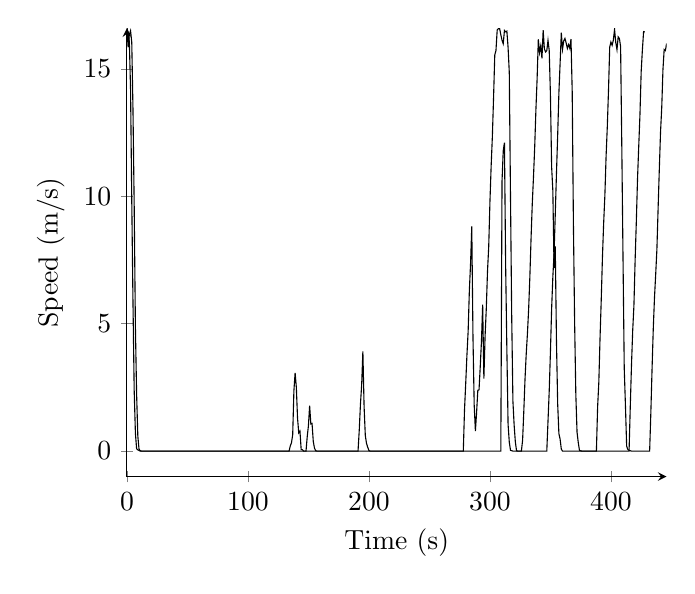
\begin{tikzpicture}
\begin{axis}[
legend style={anchor=west},
axis x line=bottom,
axis y line=left,
ymin=-1,
xlabel=Time (s),
ylabel=Speed (m/s),
]
\addplot[] coordinates {
(0, 16.6)
(1, 15.8460053715)
(2, 16.3514843297)
(3, 16.5000067825)
(4, 16.0420976826)
(5, 13.4119518313)
(6, 9.64671911235)
(7, 4.88439790454)
(8, 2.24581927001)
(9, 0.596283013476)
(10, 0.0744733324328)
(11, 0.0111308723506)
(12, 0.0)
(13, 0.0)
(14, 0.0)
(15, 0.0)
(16, 0.0)
(17, 0.0)
(18, 0.0)
(19, 0.0)
(20, 0.0)
(21, 0.0)
(22, 0.0)
(23, 0.0)
(24, 0.0)
(25, 0.0)
(26, 0.0)
(27, 0.0)
(28, 0.0)
(29, 0.0)
(30, 0.0)
(31, 0.0)
(32, 0.0)
(33, 0.0)
(34, 0.0)
(35, 0.0)
(36, 0.0)
(37, 0.0)
(38, 0.0)
(39, 0.0)
(40, 0.0)
(41, 0.0)
(42, 0.0)
(43, 0.0)
(44, 0.0)
(45, 0.0)
(46, 0.0)
(47, 0.0)
(48, 0.0)
(49, 0.0)
(50, 0.0)
(51, 0.0)
(52, 0.0)
(53, 0.0)
(54, 0.0)
(55, 0.0)
(56, 0.0)
(57, 0.0)
(58, 0.0)
(59, 0.0)
(60, 0.0)
(61, 0.0)
(62, 0.0)
(63, 0.0)
(64, 0.0)
(65, 0.0)
(66, 0.0)
(67, 0.0)
(68, 0.0)
(69, 0.0)
(70, 0.0)
(71, 0.0)
(72, 0.0)
(73, 0.0)
(74, 0.0)
(75, 0.0)
(76, 0.0)
(77, 0.0)
(78, 0.0)
(79, 0.0)
(80, 0.0)
(81, 0.0)
(82, 0.0)
(83, 0.0)
(84, 0.0)
(85, 0.0)
(86, 0.0)
(87, 0.0)
(88, 0.0)
(89, 0.0)
(90, 0.0)
(91, 0.0)
(92, 0.0)
(93, 0.0)
(94, 0.0)
(95, 0.0)
(96, 0.0)
(97, 0.0)
(98, 0.0)
(99, 0.0)
(100, 0.0)
(101, 0.0)
(102, 0.0)
(103, 0.0)
(104, 0.0)
(105, 0.0)
(106, 0.0)
(107, 0.0)
(108, 0.0)
(109, 0.0)
(110, 0.0)
(111, 0.0)
(112, 0.0)
(113, 0.0)
(114, 0.0)
(115, 0.0)
(116, 0.0)
(117, 0.0)
(118, 0.0)
(119, 0.0)
(120, 0.0)
(121, 0.0)
(122, 0.0)
(123, 0.0)
(124, 0.0)
(125, 0.0)
(126, 0.0)
(127, 0.0)
(128, 0.0)
(129, 0.0)
(130, 0.0)
(131, 0.0)
(132, 0.0)
(133, 0.0)
(134, 0.0)
(135, 0.0)
(136, 0.0)
(137, 0.0)
(138, 0.0)
(139, 0.0)
(140, 0.0)
(141, 0.0)
(142, 0.0)
(143, 0.0)
(144, 0.0)
(145, 0.0)
(146, 0.0)
(147, 0.0)
(148, 0.0)
(149, 0.0)
(150, 0.0)
(151, 0.0)
(152, 0.0)
(153, 0.0)
(154, 0.0)
(155, 0.0)
(156, 0.0)
(157, 0.0)
(158, 0.0)
(159, 0.0)
(160, 0.0)
(161, 0.0)
(162, 0.0)
(163, 0.0)
(164, 0.0)
(165, 0.0)
(166, 0.0)
(167, 0.0)
(168, 0.0)
(169, 0.0)
(170, 0.0)
(171, 0.0)
(172, 0.0)
(173, 0.0)
(174, 0.0)
(175, 0.0)
(176, 0.0)
(177, 0.0)
(178, 0.0)
(179, 0.0)
(180, 0.0)
(181, 0.0)
(182, 0.0)
(183, 0.0)
(184, 0.0)
(185, 0.0)
(186, 0.0)
(187, 0.0)
(188, 0.0)
(189, 0.0)
(190, 0.0)
(191, 0.0)
(192, 0.0)
(193, 0.0)
(194, 0.0)
(195, 0.0)
(196, 0.0)
(197, 0.0)
(198, 0.0)
(199, 0.0)
(200, 0.0)
(201, 0.0)
(202, 0.0)
(203, 0.0)
(204, 0.0)
(205, 0.0)
(206, 0.0)
(207, 0.0)
(208, 0.0)
(209, 0.0)
(210, 0.0)
(211, 0.0)
(212, 0.0)
(213, 0.0)
(214, 0.0)
(215, 0.0)
(216, 0.0)
(217, 0.0)
(218, 0.0)
(219, 0.0)
(220, 0.0)
(221, 0.0)
(222, 0.0)
(223, 0.0)
(224, 0.0)
(225, 0.0)
(226, 0.0)
(227, 0.0)
(228, 0.0)
(229, 0.0)
(230, 0.0)
(231, 0.0)
(232, 0.0)
(233, 0.0)
(234, 0.0)
(235, 0.0)
(236, 0.0)
(237, 0.0)
(238, 0.0)
(239, 0.0)
(240, 0.0)
(241, 0.0)
(242, 0.0)
(243, 0.0)
(244, 0.0)
(245, 0.0)
(246, 0.0)
(247, 0.0)
(248, 0.0)
(249, 0.0)
(250, 0.0)
(251, 0.0)
(252, 0.0)
(253, 0.0)
(254, 0.0)
(255, 0.0)
(256, 0.0)
(257, 0.0)
(258, 0.0)
(259, 0.0)
(260, 0.0)
(261, 0.0)
(262, 0.0)
(263, 0.0)
(264, 0.0)
(265, 0.0)
(266, 0.0)
(267, 0.0)
(268, 0.0)
(269, 0.0)
(270, 0.0)
(271, 0.0)
(272, 0.0)
(273, 0.0)
(274, 0.0)
(275, 0.0)
(276, 0.0)
(277, 0.0)
(278, 0.0)
(279, 0.0)
(280, 0.0)
(281, 0.0)
(282, 0.0)
(283, 0.0)
(284, 0.0)
(285, 0.0)
(286, 0.0)
(287, 0.0)
(288, 0.0)
(289, 0.0)
(290, 0.0)
(291, 0.0)
(292, 0.0)
(293, 0.0)
(294, 0.0)
(295, 0.0)
(296, 0.0)
(297, 0.0)
(298, 0.0)
(299, 0.0)
(300, 0.0)
(301, 0.0)
(302, 0.0)
(303, 0.0)
(304, 0.0)
(305, 0.0)
(306, 0.0)
(307, 0.0)
(308, 0.0)
(309, 0.0)
(310, 10.6)
(311, 11.7853389539)
(312, 12.1106115905)
(313, 7.26215271977)
(314, 3.98230663951)
(315, 1.04826378063)
(316, 0.35208487045)
(317, 0.0310439180269)
(318, 0.0156147280314)
(319, 0.0)
(320, 0.0)
(321, 0.0)
(322, 0.0)
(323, 0.0)
(324, 0.0)
(325, 0.0)
(326, 0.0)
(327, 0.420550189962)
(328, 1.56640021053)
(329, 2.8212365466)
(330, 3.81468290065)
(331, 4.60842953747)
(332, 5.56918073882)
(333, 6.83731748822)
(334, 8.35733550986)
(335, 9.70727049369)
(336, 10.7559008614)
(337, 11.9272649598)
(338, 13.3903768172)
(339, 14.6183286763)
(340, 16.1654462923)
(341, 15.6419831231)
(342, 15.9074035298)
(343, 15.4140734702)
(344, 16.5205052993)
(345, 15.7864614757)
(346, 15.669667174)
(347, 15.720357464)
(348, 16.1227902737)
(349, 15.7265084987)
(350, 13.9964047844)
(351, 11.1545525602)
(352, 10.2246152472)
(353, 7.1915703525)
(354, 8.03196345812)
(355, 4.28765076227)
(356, 1.84631470386)
(357, 0.680642151364)
(358, 0.471646837251)
(359, 0.0744557253106)
(360, 0.0)
(361, 0.0)
(362, 0.0)
(363, 0.0)
(364, 0.0)
(365, 0.0)
(366, 0.0)
(367, 0.0)
(368, 0.0)
(369, 0.0)
(370, 0.0)
(371, 0.0)
(372, 0.0)
(373, 0.0)
(374, 0.0)
(375, 0.0)
(376, 0.0)
(377, 0.0)
(378, 0.0)
(379, 0.0)
(380, 0.0)
(381, 0.0)
(382, 0.0)
(383, 0.0)
(384, 0.0)
(385, 0.0)
(386, 0.0)
(387, 0.0)
(388, 0.0)
(389, 1.72941104933)
(390, 2.70156619381)
(391, 4.43408716181)
(392, 5.93917380616)
(393, 7.61632095692)
(394, 8.95431810049)
(395, 10.0343269941)
(396, 11.568830091)
(397, 12.7215696063)
(398, 14.1630580385)
(399, 15.8624374294)
(400, 16.0565942283)
(401, 15.92837544)
(402, 16.1341139032)
(403, 16.5548182908)
(404, 16.039996413)
(405, 15.7591015432)
(406, 16.2609505742)
(407, 16.1985097619)
(408, 15.8811872716)
(409, 11.9272891521)
(410, 7.55054814463)
(411, 3.26383025473)
(412, 1.78789280029)
(413, 0.191083667377)
(414, 0.0605579549299)
(415, 0.027871491568)
(416, 0.0123929064508)
(417, 0.0)
(418, 0.0)
(419, 0.0)
(420, 0.0)
(421, 0.0)
(422, 0.0)
(423, 0.0)
(424, 0.0)
(425, 0.0)
(426, 0.0)
(427, 0.0)
(428, 0.0)
(429, 0.0)
(430, 0.0)
(431, 0.0)
(432, 0.0)
(433, 1.51256702081)
(434, 3.22975468312)
(435, 4.79953276331)
(436, 6.01897485943)
(437, 6.93787045868)
(438, 7.92591938346)
(439, 9.52968241121)
(440, 11.0705194117)
(441, 12.5272176492)
(442, 13.4876530336)
(443, 14.9753508418)
(444, 15.7629790612)
(445, 15.7230149394)
(446, 15.999285037)
};
\addplot[] coordinates {
(0, 16.6)
(1, 16.4063530304)
(2, 16.0686071615)
(3, 14.2046453239)
(4, 9.81354509882)
(5, 5.85064829607)
(6, 2.37143876284)
(7, 0.709744663937)
(8, 0.0909120592065)
(9, 0.0485784264072)
(10, 0.021748766261)
(11, 0.0)
(12, 0.0)
(13, 0.0)
(14, 0.0)
(15, 0.0)
(16, 0.0)
(17, 0.0)
(18, 0.0)
(19, 0.0)
(20, 0.0)
(21, 0.0)
(22, 0.0)
(23, 0.0)
(24, 0.0)
(25, 0.0)
(26, 0.0)
(27, 0.0)
(28, 0.0)
(29, 0.0)
(30, 0.0)
(31, 0.0)
(32, 0.0)
(33, 0.0)
(34, 0.0)
(35, 0.0)
(36, 0.0)
(37, 0.0)
(38, 0.0)
(39, 0.0)
(40, 0.0)
(41, 0.0)
(42, 0.0)
(43, 0.0)
(44, 0.0)
(45, 0.0)
(46, 0.0)
(47, 0.0)
(48, 0.0)
(49, 0.0)
(50, 0.0)
(51, 0.0)
(52, 0.0)
(53, 0.0)
(54, 0.0)
(55, 0.0)
(56, 0.0)
(57, 0.0)
(58, 0.0)
(59, 0.0)
(60, 0.0)
(61, 0.0)
(62, 0.0)
(63, 0.0)
(64, 0.0)
(65, 0.0)
(66, 0.0)
(67, 0.0)
(68, 0.0)
(69, 0.0)
(70, 0.0)
(71, 0.0)
(72, 0.0)
(73, 0.0)
(74, 0.0)
(75, 0.0)
(76, 0.0)
(77, 0.0)
(78, 0.0)
(79, 0.0)
(80, 0.0)
(81, 0.0)
(82, 0.0)
(83, 0.0)
(84, 0.0)
(85, 0.0)
(86, 0.0)
(87, 0.0)
(88, 0.0)
(89, 0.0)
(90, 0.0)
(91, 0.0)
(92, 0.0)
(93, 0.0)
(94, 0.0)
(95, 0.0)
(96, 0.0)
(97, 0.0)
(98, 0.0)
(99, 0.0)
(100, 0.0)
(101, 0.0)
(102, 0.0)
(103, 0.0)
(104, 0.0)
(105, 0.0)
(106, 0.0)
(107, 0.0)
(108, 0.0)
(109, 0.0)
(110, 0.0)
(111, 0.0)
(112, 0.0)
(113, 0.0)
(114, 0.0)
(115, 0.0)
(116, 0.0)
(117, 0.0)
(118, 0.0)
(119, 0.0)
(120, 0.0)
(121, 0.0)
(122, 0.0)
(123, 0.0)
(124, 0.0)
(125, 0.0)
(126, 0.0)
(127, 0.0)
(128, 0.0)
(129, 0.0)
(130, 0.0)
(131, 0.0)
(132, 0.0)
(133, 0.0)
(134, 0.0)
(135, 0.201348355256)
(136, 0.325494695873)
(137, 0.643656041027)
(138, 2.36801344039)
(139, 3.07268509555)
(140, 2.51097225038)
(141, 1.29404918741)
(142, 0.712911094816)
(143, 0.782451475589)
(144, 0.059962655217)
(145, 0.0538438149298)
(146, 0.0)
(147, 0.0)
(148, 0.0)
(149, 0.559835290344)
(150, 0.996451556731)
(151, 1.78431083768)
(152, 1.06077898319)
(153, 1.0809598356)
(154, 0.382455471683)
(155, 0.11543004073)
(156, 0.0152610706536)
(157, 0.0)
(158, 0.0)
(159, 0.0)
(160, 0.0)
(161, 0.0)
(162, 0.0)
(163, 0.0)
(164, 0.0)
(165, 0.0)
(166, 0.0)
(167, 0.0)
(168, 0.0)
(169, 0.0)
(170, 0.0)
(171, 0.0)
(172, 0.0)
(173, 0.0)
(174, 0.0)
(175, 0.0)
(176, 0.0)
(177, 0.0)
(178, 0.0)
(179, 0.0)
(180, 0.0)
(181, 0.0)
(182, 0.0)
(183, 0.0)
(184, 0.0)
(185, 0.0)
(186, 0.0)
(187, 0.0)
(188, 0.0)
(189, 0.0)
(190, 0.0)
(191, 0.0)
(192, 0.814360254376)
(193, 1.84453541419)
(194, 2.5970048068)
(195, 3.91208518568)
(196, 1.75092969831)
(197, 0.616202946931)
(198, 0.299305872288)
(199, 0.152474668227)
(200, 0.0214985522599)
(201, 0.0)
(202, 0.0)
(203, 0.0)
(204, 0.0)
(205, 0.0)
(206, 0.0)
(207, 0.0)
(208, 0.0)
(209, 0.0)
(210, 0.0)
(211, 0.0)
(212, 0.0)
(213, 0.0)
(214, 0.0)
(215, 0.0)
(216, 0.0)
(217, 0.0)
(218, 0.0)
(219, 0.0)
(220, 0.0)
(221, 0.0)
(222, 0.0)
(223, 0.0)
(224, 0.0)
(225, 0.0)
(226, 0.0)
(227, 0.0)
(228, 0.0)
(229, 0.0)
(230, 0.0)
(231, 0.0)
(232, 0.0)
(233, 0.0)
(234, 0.0)
(235, 0.0)
(236, 0.0)
(237, 0.0)
(238, 0.0)
(239, 0.0)
(240, 0.0)
(241, 0.0)
(242, 0.0)
(243, 0.0)
(244, 0.0)
(245, 0.0)
(246, 0.0)
(247, 0.0)
(248, 0.0)
(249, 0.0)
(250, 0.0)
(251, 0.0)
(252, 0.0)
(253, 0.0)
(254, 0.0)
(255, 0.0)
(256, 0.0)
(257, 0.0)
(258, 0.0)
(259, 0.0)
(260, 0.0)
(261, 0.0)
(262, 0.0)
(263, 0.0)
(264, 0.0)
(265, 0.0)
(266, 0.0)
(267, 0.0)
(268, 0.0)
(269, 0.0)
(270, 0.0)
(271, 0.0)
(272, 0.0)
(273, 0.0)
(274, 0.0)
(275, 0.0)
(276, 0.0)
(277, 0.0)
(278, 0.0)
(279, 1.62045613818)
(280, 2.66695256182)
(281, 3.76390033895)
(282, 4.70575594094)
(283, 6.29156046475)
(284, 7.3642949007)
(285, 8.82025540248)
(286, 4.45172426382)
(287, 1.80336822841)
(288, 0.786812070177)
(289, 1.53032306586)
(290, 2.38744647375)
(291, 2.40495287824)
(292, 3.31741629005)
(293, 4.30404455983)
(294, 5.74684656479)
(295, 2.84383353413)
(296, 4.50791155902)
(297, 5.5956094714)
(298, 7.05850430262)
(299, 8.02222097091)
(300, 9.76679595533)
(301, 11.1745537445)
(302, 12.3267531638)
(303, 13.8623859471)
(304, 15.5467238072)
(305, 15.728478375)
(306, 16.5276059214)
(307, 16.5840379973)
(308, 16.5887493624)
(309, 16.34461902)
(310, 16.1304618118)
(311, 15.9917063138)
(312, 16.5106300041)
(313, 16.4582202713)
(314, 16.4874577963)
(315, 15.850714892)
(316, 14.8667659929)
(317, 10.0017729302)
(318, 5.29738886009)
(319, 1.96481926838)
(320, 1.03002543727)
(321, 0.3654416395)
(322, 0.0103591407087)
(323, 0.0)
(324, 0.0)
(325, 0.0)
(326, 0.0)
(327, 0.0)
(328, 0.0)
(329, 0.0)
(330, 0.0)
(331, 0.0)
(332, 0.0)
(333, 0.0)
(334, 0.0)
(335, 0.0)
(336, 0.0)
(337, 0.0)
(338, 0.0)
(339, 0.0)
(340, 0.0)
(341, 0.0)
(342, 0.0)
(343, 0.0)
(344, 0.0)
(345, 0.0)
(346, 0.0)
(347, 0.0)
(348, 1.17577672871)
(349, 2.34806267952)
(350, 3.87925270668)
(351, 5.59073773047)
(352, 6.83699818554)
(353, 7.74307288521)
(354, 9.29233657988)
(355, 10.9066890784)
(356, 12.4124361715)
(357, 14.062749687)
(358, 15.2241291486)
(359, 16.4241127164)
(360, 15.7738242253)
(361, 16.1026649337)
(362, 16.2006037558)
(363, 16.0197037247)
(364, 15.806818411)
(365, 15.9568461826)
(366, 15.8138234788)
(367, 16.1743724886)
(368, 14.121146955)
(369, 8.93044848744)
(370, 5.0571764702)
(371, 2.20926125776)
(372, 0.738937160179)
(373, 0.337602451978)
(374, 0.030457680075)
(375, 0.00994756587087)
(376, 0.0)
(377, 0.0)
(378, 0.0)
(379, 0.0)
(380, 0.0)
(381, 0.0)
(382, 0.0)
(383, 0.0)
(384, 0.0)
(385, 0.0)
(386, 0.0)
(387, 0.0)
(388, 0.0)
(389, 0.0)
(390, 0.0)
(391, 0.0)
(392, 0.0)
(393, 0.0)
(394, 0.0)
(395, 0.0)
(396, 0.0)
(397, 0.0)
(398, 0.0)
(399, 0.0)
(400, 0.0)
(401, 0.0)
(402, 0.0)
(403, 0.0)
(404, 0.0)
(405, 0.0)
(406, 0.0)
(407, 0.0)
(408, 0.0)
(409, 0.0)
(410, 0.0)
(411, 0.0)
(412, 0.0)
(413, 0.0)
(414, 0.0)
(415, 0.0)
(416, 1.75659008157)
(417, 3.38026934776)
(418, 4.73459405084)
(419, 5.69919825748)
(420, 7.4948383546)
(421, 9.01964666911)
(422, 10.7083133994)
(423, 11.984823914)
(424, 13.2165782051)
(425, 14.8907359817)
(426, 15.7435259929)
(427, 16.4661744598)
(428, 16.4521838746)
};

\end{axis}
\end{tikzpicture}
\label{tik:speed:0:51}
\caption{0 percent diving with GSC on route $51$}
\end{figure}

%
\begin{figure}
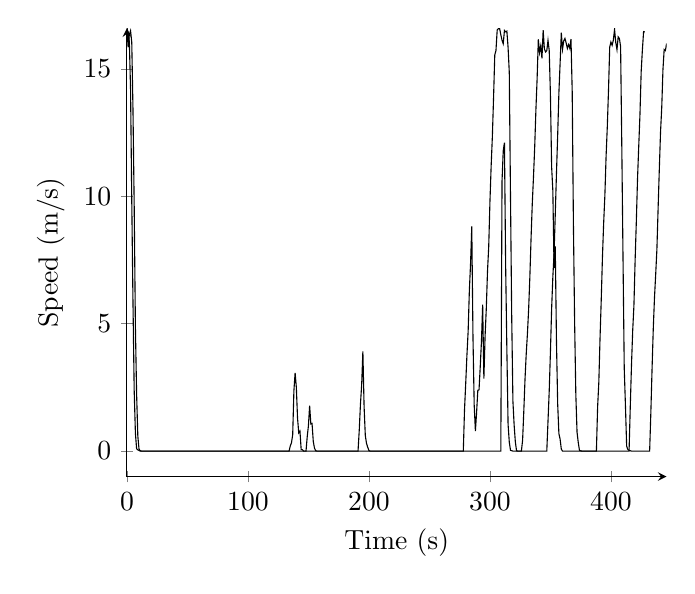
\begin{tikzpicture}
\begin{axis}[
legend style={anchor=west},
axis x line=bottom,
axis y line=left,
ymin=-1,
xlabel=Time (s),
ylabel=Speed (m/s),
]
\addplot[] coordinates {
(0, 16.6)
(1, 15.8460053715)
(2, 16.3514843297)
(3, 16.5000067825)
(4, 16.0420976826)
(5, 13.4119518313)
(6, 9.64671911235)
(7, 4.88439790454)
(8, 2.24581927001)
(9, 0.596283013476)
(10, 0.0744733324328)
(11, 0.0111308723506)
(12, 0.0)
(13, 0.0)
(14, 0.0)
(15, 0.0)
(16, 0.0)
(17, 0.0)
(18, 0.0)
(19, 0.0)
(20, 0.0)
(21, 0.0)
(22, 0.0)
(23, 0.0)
(24, 0.0)
(25, 0.0)
(26, 0.0)
(27, 0.0)
(28, 0.0)
(29, 0.0)
(30, 0.0)
(31, 0.0)
(32, 0.0)
(33, 0.0)
(34, 0.0)
(35, 0.0)
(36, 0.0)
(37, 0.0)
(38, 0.0)
(39, 0.0)
(40, 0.0)
(41, 0.0)
(42, 0.0)
(43, 0.0)
(44, 0.0)
(45, 0.0)
(46, 0.0)
(47, 0.0)
(48, 0.0)
(49, 0.0)
(50, 0.0)
(51, 0.0)
(52, 0.0)
(53, 0.0)
(54, 0.0)
(55, 0.0)
(56, 0.0)
(57, 0.0)
(58, 0.0)
(59, 0.0)
(60, 0.0)
(61, 0.0)
(62, 0.0)
(63, 0.0)
(64, 0.0)
(65, 0.0)
(66, 0.0)
(67, 0.0)
(68, 0.0)
(69, 0.0)
(70, 0.0)
(71, 0.0)
(72, 0.0)
(73, 0.0)
(74, 0.0)
(75, 0.0)
(76, 0.0)
(77, 0.0)
(78, 0.0)
(79, 0.0)
(80, 0.0)
(81, 0.0)
(82, 0.0)
(83, 0.0)
(84, 0.0)
(85, 0.0)
(86, 0.0)
(87, 0.0)
(88, 0.0)
(89, 0.0)
(90, 0.0)
(91, 0.0)
(92, 0.0)
(93, 0.0)
(94, 0.0)
(95, 0.0)
(96, 0.0)
(97, 0.0)
(98, 0.0)
(99, 0.0)
(100, 0.0)
(101, 0.0)
(102, 0.0)
(103, 0.0)
(104, 0.0)
(105, 0.0)
(106, 0.0)
(107, 0.0)
(108, 0.0)
(109, 0.0)
(110, 0.0)
(111, 0.0)
(112, 0.0)
(113, 0.0)
(114, 0.0)
(115, 0.0)
(116, 0.0)
(117, 0.0)
(118, 0.0)
(119, 0.0)
(120, 0.0)
(121, 0.0)
(122, 0.0)
(123, 0.0)
(124, 0.0)
(125, 0.0)
(126, 0.0)
(127, 0.0)
(128, 0.0)
(129, 0.0)
(130, 0.0)
(131, 0.0)
(132, 0.0)
(133, 0.0)
(134, 0.0)
(135, 0.0)
(136, 0.0)
(137, 0.0)
(138, 0.0)
(139, 0.0)
(140, 0.0)
(141, 0.0)
(142, 0.0)
(143, 0.0)
(144, 0.0)
(145, 0.0)
(146, 0.0)
(147, 0.0)
(148, 0.0)
(149, 0.0)
(150, 0.0)
(151, 0.0)
(152, 0.0)
(153, 0.0)
(154, 0.0)
(155, 0.0)
(156, 0.0)
(157, 0.0)
(158, 0.0)
(159, 0.0)
(160, 0.0)
(161, 0.0)
(162, 0.0)
(163, 0.0)
(164, 0.0)
(165, 0.0)
(166, 0.0)
(167, 0.0)
(168, 0.0)
(169, 0.0)
(170, 0.0)
(171, 0.0)
(172, 0.0)
(173, 0.0)
(174, 0.0)
(175, 0.0)
(176, 0.0)
(177, 0.0)
(178, 0.0)
(179, 0.0)
(180, 0.0)
(181, 0.0)
(182, 0.0)
(183, 0.0)
(184, 0.0)
(185, 0.0)
(186, 0.0)
(187, 0.0)
(188, 0.0)
(189, 0.0)
(190, 0.0)
(191, 0.0)
(192, 0.0)
(193, 0.0)
(194, 0.0)
(195, 0.0)
(196, 0.0)
(197, 0.0)
(198, 0.0)
(199, 0.0)
(200, 0.0)
(201, 0.0)
(202, 0.0)
(203, 0.0)
(204, 0.0)
(205, 0.0)
(206, 0.0)
(207, 0.0)
(208, 0.0)
(209, 0.0)
(210, 0.0)
(211, 0.0)
(212, 0.0)
(213, 0.0)
(214, 0.0)
(215, 0.0)
(216, 0.0)
(217, 0.0)
(218, 0.0)
(219, 0.0)
(220, 0.0)
(221, 0.0)
(222, 0.0)
(223, 0.0)
(224, 0.0)
(225, 0.0)
(226, 0.0)
(227, 0.0)
(228, 0.0)
(229, 0.0)
(230, 0.0)
(231, 0.0)
(232, 0.0)
(233, 0.0)
(234, 0.0)
(235, 0.0)
(236, 0.0)
(237, 0.0)
(238, 0.0)
(239, 0.0)
(240, 0.0)
(241, 0.0)
(242, 0.0)
(243, 0.0)
(244, 0.0)
(245, 0.0)
(246, 0.0)
(247, 0.0)
(248, 0.0)
(249, 0.0)
(250, 0.0)
(251, 0.0)
(252, 0.0)
(253, 0.0)
(254, 0.0)
(255, 0.0)
(256, 0.0)
(257, 0.0)
(258, 0.0)
(259, 0.0)
(260, 0.0)
(261, 0.0)
(262, 0.0)
(263, 0.0)
(264, 0.0)
(265, 0.0)
(266, 0.0)
(267, 0.0)
(268, 0.0)
(269, 0.0)
(270, 0.0)
(271, 0.0)
(272, 0.0)
(273, 0.0)
(274, 0.0)
(275, 0.0)
(276, 0.0)
(277, 0.0)
(278, 0.0)
(279, 0.0)
(280, 0.0)
(281, 0.0)
(282, 0.0)
(283, 0.0)
(284, 0.0)
(285, 0.0)
(286, 0.0)
(287, 0.0)
(288, 0.0)
(289, 0.0)
(290, 0.0)
(291, 0.0)
(292, 0.0)
(293, 0.0)
(294, 0.0)
(295, 0.0)
(296, 0.0)
(297, 0.0)
(298, 0.0)
(299, 0.0)
(300, 0.0)
(301, 0.0)
(302, 0.0)
(303, 0.0)
(304, 0.0)
(305, 0.0)
(306, 0.0)
(307, 0.0)
(308, 0.0)
(309, 0.0)
(310, 10.6)
(311, 11.7853389539)
(312, 12.1106115905)
(313, 7.26215271977)
(314, 3.98230663951)
(315, 1.04826378063)
(316, 0.35208487045)
(317, 0.0310439180269)
(318, 0.0156147280314)
(319, 0.0)
(320, 0.0)
(321, 0.0)
(322, 0.0)
(323, 0.0)
(324, 0.0)
(325, 0.0)
(326, 0.0)
(327, 0.420550189962)
(328, 1.56640021053)
(329, 2.8212365466)
(330, 3.81468290065)
(331, 4.60842953747)
(332, 5.56918073882)
(333, 6.83731748822)
(334, 8.35733550986)
(335, 9.70727049369)
(336, 10.7559008614)
(337, 11.9272649598)
(338, 13.3903768172)
(339, 14.6183286763)
(340, 16.1654462923)
(341, 15.6419831231)
(342, 15.9074035298)
(343, 15.4140734702)
(344, 16.5205052993)
(345, 15.7864614757)
(346, 15.669667174)
(347, 15.720357464)
(348, 16.1227902737)
(349, 15.7265084987)
(350, 13.9964047844)
(351, 11.1545525602)
(352, 10.2246152472)
(353, 7.1915703525)
(354, 8.03196345812)
(355, 4.28765076227)
(356, 1.84631470386)
(357, 0.680642151364)
(358, 0.471646837251)
(359, 0.0744557253106)
(360, 0.0)
(361, 0.0)
(362, 0.0)
(363, 0.0)
(364, 0.0)
(365, 0.0)
(366, 0.0)
(367, 0.0)
(368, 0.0)
(369, 0.0)
(370, 0.0)
(371, 0.0)
(372, 0.0)
(373, 0.0)
(374, 0.0)
(375, 0.0)
(376, 0.0)
(377, 0.0)
(378, 0.0)
(379, 0.0)
(380, 0.0)
(381, 0.0)
(382, 0.0)
(383, 0.0)
(384, 0.0)
(385, 0.0)
(386, 0.0)
(387, 0.0)
(388, 0.0)
(389, 1.72941104933)
(390, 2.70156619381)
(391, 4.43408716181)
(392, 5.93917380616)
(393, 7.61632095692)
(394, 8.95431810049)
(395, 10.0343269941)
(396, 11.568830091)
(397, 12.7215696063)
(398, 14.1630580385)
(399, 15.8624374294)
(400, 16.0565942283)
(401, 15.92837544)
(402, 16.1341139032)
(403, 16.5548182908)
(404, 16.039996413)
(405, 15.7591015432)
(406, 16.2609505742)
(407, 16.1985097619)
(408, 15.8811872716)
(409, 11.9272891521)
(410, 7.55054814463)
(411, 3.26383025473)
(412, 1.78789280029)
(413, 0.191083667377)
(414, 0.0605579549299)
(415, 0.027871491568)
(416, 0.0123929064508)
(417, 0.0)
(418, 0.0)
(419, 0.0)
(420, 0.0)
(421, 0.0)
(422, 0.0)
(423, 0.0)
(424, 0.0)
(425, 0.0)
(426, 0.0)
(427, 0.0)
(428, 0.0)
(429, 0.0)
(430, 0.0)
(431, 0.0)
(432, 0.0)
(433, 1.51256702081)
(434, 3.22975468312)
(435, 4.79953276331)
(436, 6.01897485943)
(437, 6.93787045868)
(438, 7.92591938346)
(439, 9.52968241121)
(440, 11.0705194117)
(441, 12.5272176492)
(442, 13.4876530336)
(443, 14.9753508418)
(444, 15.7629790612)
(445, 15.7230149394)
(446, 15.999285037)
};
\addplot[] coordinates {
(0, 16.6)
(1, 16.4063530304)
(2, 16.0686071615)
(3, 14.2046453239)
(4, 9.81354509882)
(5, 5.85064829607)
(6, 2.37143876284)
(7, 0.709744663937)
(8, 0.0909120592065)
(9, 0.0485784264072)
(10, 0.021748766261)
(11, 0.0)
(12, 0.0)
(13, 0.0)
(14, 0.0)
(15, 0.0)
(16, 0.0)
(17, 0.0)
(18, 0.0)
(19, 0.0)
(20, 0.0)
(21, 0.0)
(22, 0.0)
(23, 0.0)
(24, 0.0)
(25, 0.0)
(26, 0.0)
(27, 0.0)
(28, 0.0)
(29, 0.0)
(30, 0.0)
(31, 0.0)
(32, 0.0)
(33, 0.0)
(34, 0.0)
(35, 0.0)
(36, 0.0)
(37, 0.0)
(38, 0.0)
(39, 0.0)
(40, 0.0)
(41, 0.0)
(42, 0.0)
(43, 0.0)
(44, 0.0)
(45, 0.0)
(46, 0.0)
(47, 0.0)
(48, 0.0)
(49, 0.0)
(50, 0.0)
(51, 0.0)
(52, 0.0)
(53, 0.0)
(54, 0.0)
(55, 0.0)
(56, 0.0)
(57, 0.0)
(58, 0.0)
(59, 0.0)
(60, 0.0)
(61, 0.0)
(62, 0.0)
(63, 0.0)
(64, 0.0)
(65, 0.0)
(66, 0.0)
(67, 0.0)
(68, 0.0)
(69, 0.0)
(70, 0.0)
(71, 0.0)
(72, 0.0)
(73, 0.0)
(74, 0.0)
(75, 0.0)
(76, 0.0)
(77, 0.0)
(78, 0.0)
(79, 0.0)
(80, 0.0)
(81, 0.0)
(82, 0.0)
(83, 0.0)
(84, 0.0)
(85, 0.0)
(86, 0.0)
(87, 0.0)
(88, 0.0)
(89, 0.0)
(90, 0.0)
(91, 0.0)
(92, 0.0)
(93, 0.0)
(94, 0.0)
(95, 0.0)
(96, 0.0)
(97, 0.0)
(98, 0.0)
(99, 0.0)
(100, 0.0)
(101, 0.0)
(102, 0.0)
(103, 0.0)
(104, 0.0)
(105, 0.0)
(106, 0.0)
(107, 0.0)
(108, 0.0)
(109, 0.0)
(110, 0.0)
(111, 0.0)
(112, 0.0)
(113, 0.0)
(114, 0.0)
(115, 0.0)
(116, 0.0)
(117, 0.0)
(118, 0.0)
(119, 0.0)
(120, 0.0)
(121, 0.0)
(122, 0.0)
(123, 0.0)
(124, 0.0)
(125, 0.0)
(126, 0.0)
(127, 0.0)
(128, 0.0)
(129, 0.0)
(130, 0.0)
(131, 0.0)
(132, 0.0)
(133, 0.0)
(134, 0.0)
(135, 0.201348355256)
(136, 0.325494695873)
(137, 0.643656041027)
(138, 2.36801344039)
(139, 3.07268509555)
(140, 2.51097225038)
(141, 1.29404918741)
(142, 0.712911094816)
(143, 0.782451475589)
(144, 0.059962655217)
(145, 0.0538438149298)
(146, 0.0)
(147, 0.0)
(148, 0.0)
(149, 0.559835290344)
(150, 0.996451556731)
(151, 1.78431083768)
(152, 1.06077898319)
(153, 1.0809598356)
(154, 0.382455471683)
(155, 0.11543004073)
(156, 0.0152610706536)
(157, 0.0)
(158, 0.0)
(159, 0.0)
(160, 0.0)
(161, 0.0)
(162, 0.0)
(163, 0.0)
(164, 0.0)
(165, 0.0)
(166, 0.0)
(167, 0.0)
(168, 0.0)
(169, 0.0)
(170, 0.0)
(171, 0.0)
(172, 0.0)
(173, 0.0)
(174, 0.0)
(175, 0.0)
(176, 0.0)
(177, 0.0)
(178, 0.0)
(179, 0.0)
(180, 0.0)
(181, 0.0)
(182, 0.0)
(183, 0.0)
(184, 0.0)
(185, 0.0)
(186, 0.0)
(187, 0.0)
(188, 0.0)
(189, 0.0)
(190, 0.0)
(191, 0.0)
(192, 0.814360254376)
(193, 1.84453541419)
(194, 2.5970048068)
(195, 3.91208518568)
(196, 1.75092969831)
(197, 0.616202946931)
(198, 0.299305872288)
(199, 0.152474668227)
(200, 0.0214985522599)
(201, 0.0)
(202, 0.0)
(203, 0.0)
(204, 0.0)
(205, 0.0)
(206, 0.0)
(207, 0.0)
(208, 0.0)
(209, 0.0)
(210, 0.0)
(211, 0.0)
(212, 0.0)
(213, 0.0)
(214, 0.0)
(215, 0.0)
(216, 0.0)
(217, 0.0)
(218, 0.0)
(219, 0.0)
(220, 0.0)
(221, 0.0)
(222, 0.0)
(223, 0.0)
(224, 0.0)
(225, 0.0)
(226, 0.0)
(227, 0.0)
(228, 0.0)
(229, 0.0)
(230, 0.0)
(231, 0.0)
(232, 0.0)
(233, 0.0)
(234, 0.0)
(235, 0.0)
(236, 0.0)
(237, 0.0)
(238, 0.0)
(239, 0.0)
(240, 0.0)
(241, 0.0)
(242, 0.0)
(243, 0.0)
(244, 0.0)
(245, 0.0)
(246, 0.0)
(247, 0.0)
(248, 0.0)
(249, 0.0)
(250, 0.0)
(251, 0.0)
(252, 0.0)
(253, 0.0)
(254, 0.0)
(255, 0.0)
(256, 0.0)
(257, 0.0)
(258, 0.0)
(259, 0.0)
(260, 0.0)
(261, 0.0)
(262, 0.0)
(263, 0.0)
(264, 0.0)
(265, 0.0)
(266, 0.0)
(267, 0.0)
(268, 0.0)
(269, 0.0)
(270, 0.0)
(271, 0.0)
(272, 0.0)
(273, 0.0)
(274, 0.0)
(275, 0.0)
(276, 0.0)
(277, 0.0)
(278, 0.0)
(279, 1.62045613818)
(280, 2.66695256182)
(281, 3.76390033895)
(282, 4.70575594094)
(283, 6.29156046475)
(284, 7.3642949007)
(285, 8.82025540248)
(286, 4.45172426382)
(287, 1.80336822841)
(288, 0.786812070177)
(289, 1.53032306586)
(290, 2.38744647375)
(291, 2.40495287824)
(292, 3.31741629005)
(293, 4.30404455983)
(294, 5.74684656479)
(295, 2.84383353413)
(296, 4.50791155902)
(297, 5.5956094714)
(298, 7.05850430262)
(299, 8.02222097091)
(300, 9.76679595533)
(301, 11.1745537445)
(302, 12.3267531638)
(303, 13.8623859471)
(304, 15.5467238072)
(305, 15.728478375)
(306, 16.5276059214)
(307, 16.5840379973)
(308, 16.5887493624)
(309, 16.34461902)
(310, 16.1304618118)
(311, 15.9917063138)
(312, 16.5106300041)
(313, 16.4582202713)
(314, 16.4874577963)
(315, 15.850714892)
(316, 14.8667659929)
(317, 10.0017729302)
(318, 5.29738886009)
(319, 1.96481926838)
(320, 1.03002543727)
(321, 0.3654416395)
(322, 0.0103591407087)
(323, 0.0)
(324, 0.0)
(325, 0.0)
(326, 0.0)
(327, 0.0)
(328, 0.0)
(329, 0.0)
(330, 0.0)
(331, 0.0)
(332, 0.0)
(333, 0.0)
(334, 0.0)
(335, 0.0)
(336, 0.0)
(337, 0.0)
(338, 0.0)
(339, 0.0)
(340, 0.0)
(341, 0.0)
(342, 0.0)
(343, 0.0)
(344, 0.0)
(345, 0.0)
(346, 0.0)
(347, 0.0)
(348, 1.17577672871)
(349, 2.34806267952)
(350, 3.87925270668)
(351, 5.59073773047)
(352, 6.83699818554)
(353, 7.74307288521)
(354, 9.29233657988)
(355, 10.9066890784)
(356, 12.4124361715)
(357, 14.062749687)
(358, 15.2241291486)
(359, 16.4241127164)
(360, 15.7738242253)
(361, 16.1026649337)
(362, 16.2006037558)
(363, 16.0197037247)
(364, 15.806818411)
(365, 15.9568461826)
(366, 15.8138234788)
(367, 16.1743724886)
(368, 14.121146955)
(369, 8.93044848744)
(370, 5.0571764702)
(371, 2.20926125776)
(372, 0.738937160179)
(373, 0.337602451978)
(374, 0.030457680075)
(375, 0.00994756587087)
(376, 0.0)
(377, 0.0)
(378, 0.0)
(379, 0.0)
(380, 0.0)
(381, 0.0)
(382, 0.0)
(383, 0.0)
(384, 0.0)
(385, 0.0)
(386, 0.0)
(387, 0.0)
(388, 0.0)
(389, 0.0)
(390, 0.0)
(391, 0.0)
(392, 0.0)
(393, 0.0)
(394, 0.0)
(395, 0.0)
(396, 0.0)
(397, 0.0)
(398, 0.0)
(399, 0.0)
(400, 0.0)
(401, 0.0)
(402, 0.0)
(403, 0.0)
(404, 0.0)
(405, 0.0)
(406, 0.0)
(407, 0.0)
(408, 0.0)
(409, 0.0)
(410, 0.0)
(411, 0.0)
(412, 0.0)
(413, 0.0)
(414, 0.0)
(415, 0.0)
(416, 1.75659008157)
(417, 3.38026934776)
(418, 4.73459405084)
(419, 5.69919825748)
(420, 7.4948383546)
(421, 9.01964666911)
(422, 10.7083133994)
(423, 11.984823914)
(424, 13.2165782051)
(425, 14.8907359817)
(426, 15.7435259929)
(427, 16.4661744598)
(428, 16.4521838746)
};

\end{axis}
\end{tikzpicture}
\label{tik:speed:0:51}
\caption{0 percent diving with GSC on route $51$}
\end{figure}


\subsection{Time}
It is interesting to investigate wether driving after \tech results in longer travel time than without.
It takes on average 114 seconds to drive a route in our test without \tech, and when all vehicles drive with \tech it takes 111 seconds. 
We therefore do not see any significant differens in thees results.


